\newcommand{\ssection}[1]{\addcontentsline{toc}{subsection}{#1, }
\subsection*{#1}%
}%

{\setbeamertemplate{footline}{\usebeamertemplate*{minimal footline}}%
\begin{frame}
    \frametitle{Outline}%
	\tableofcontents%
\end{frame}%
}%


\section{Introduction}%
\ssection{Molecular Electronics}
\begin{frame}
    \frametitle{Molecular Junction}
    \begin{figure}[!b] 
        \centering
        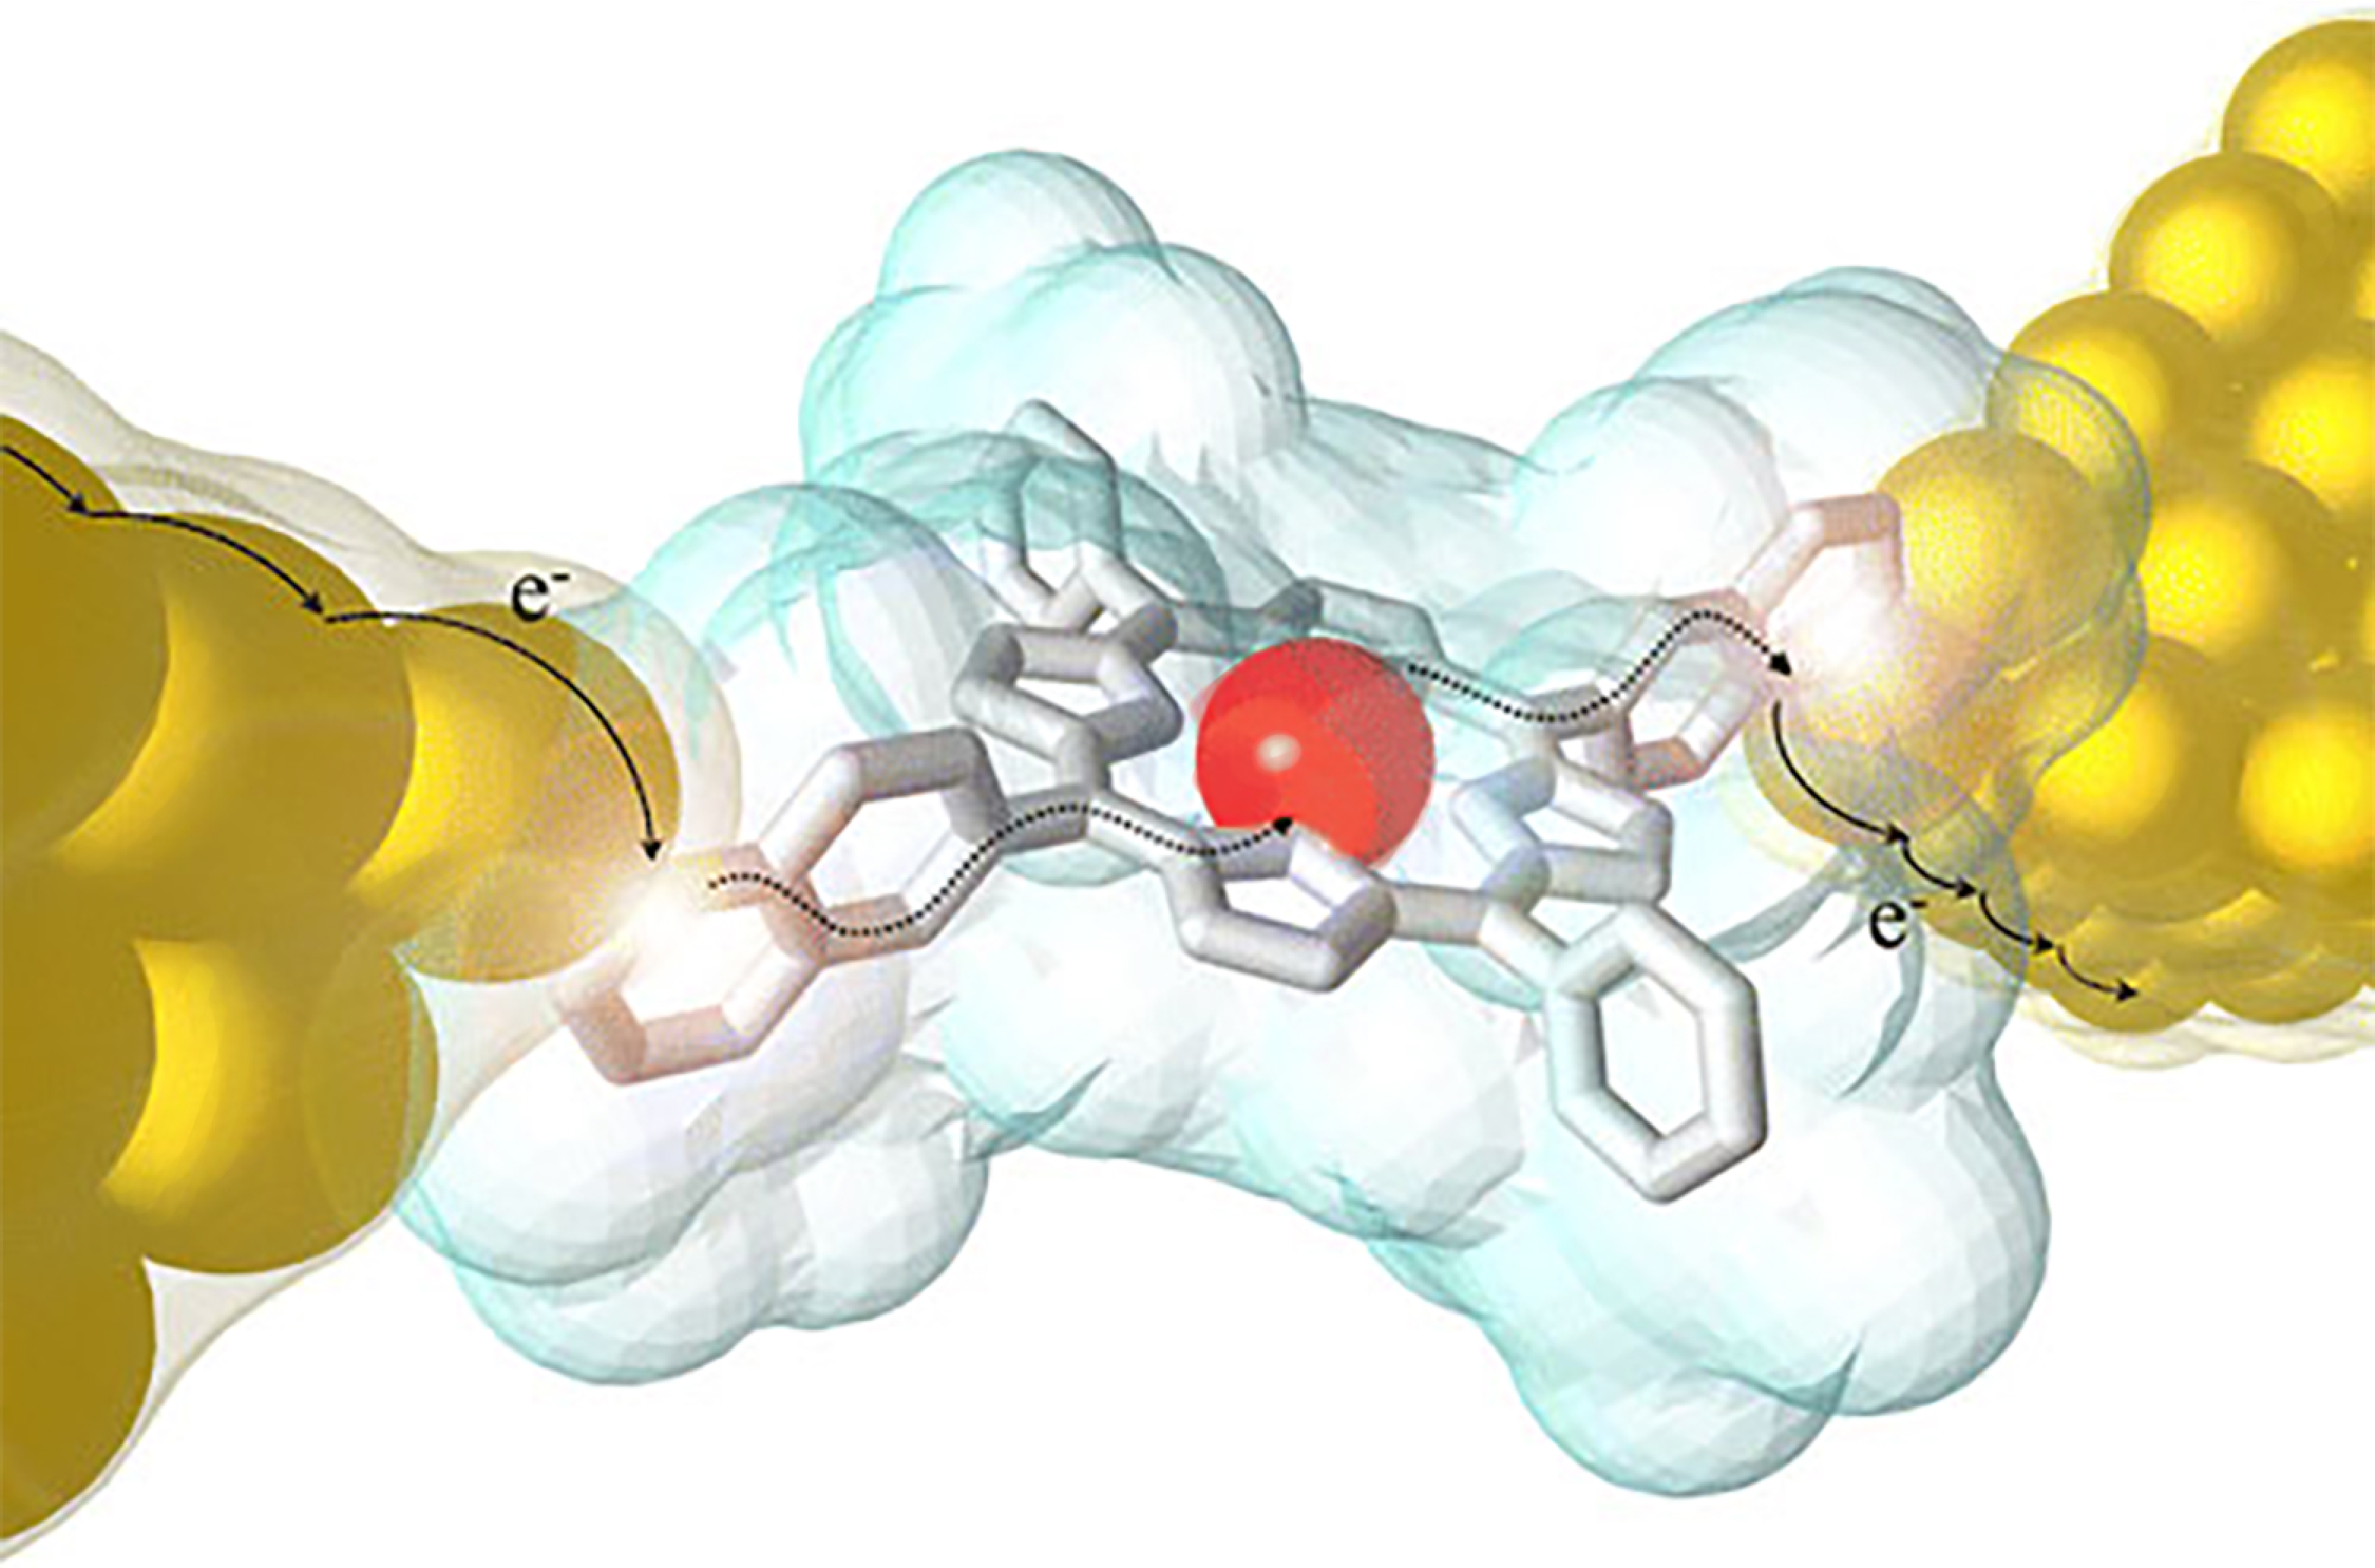
\includegraphics[height=0.5\textheight]{fig/junction.pdf}
        \caption{Artist impression of a  molecular junction. Via ~\citet{junction}.}
    \end{figure} 
\end{frame}%
\ssection{Green's Functions (Analogy)}
\begin{frame}
    \frametitle{Waves}
    \begin{figure}[!b] 
        \centering
        \includegraphics[height=0.5\textheight]{fig/wavepatterns.pdf}
        \caption{Interfering circular wave patterns (left) and fluorescent algae lightening up the wave crests (right).}
    \end{figure} 
\end{frame}%
\begin{frame}
    \frametitle{A music instrument.}
    \begin{figure}[!b] 
        \centering
        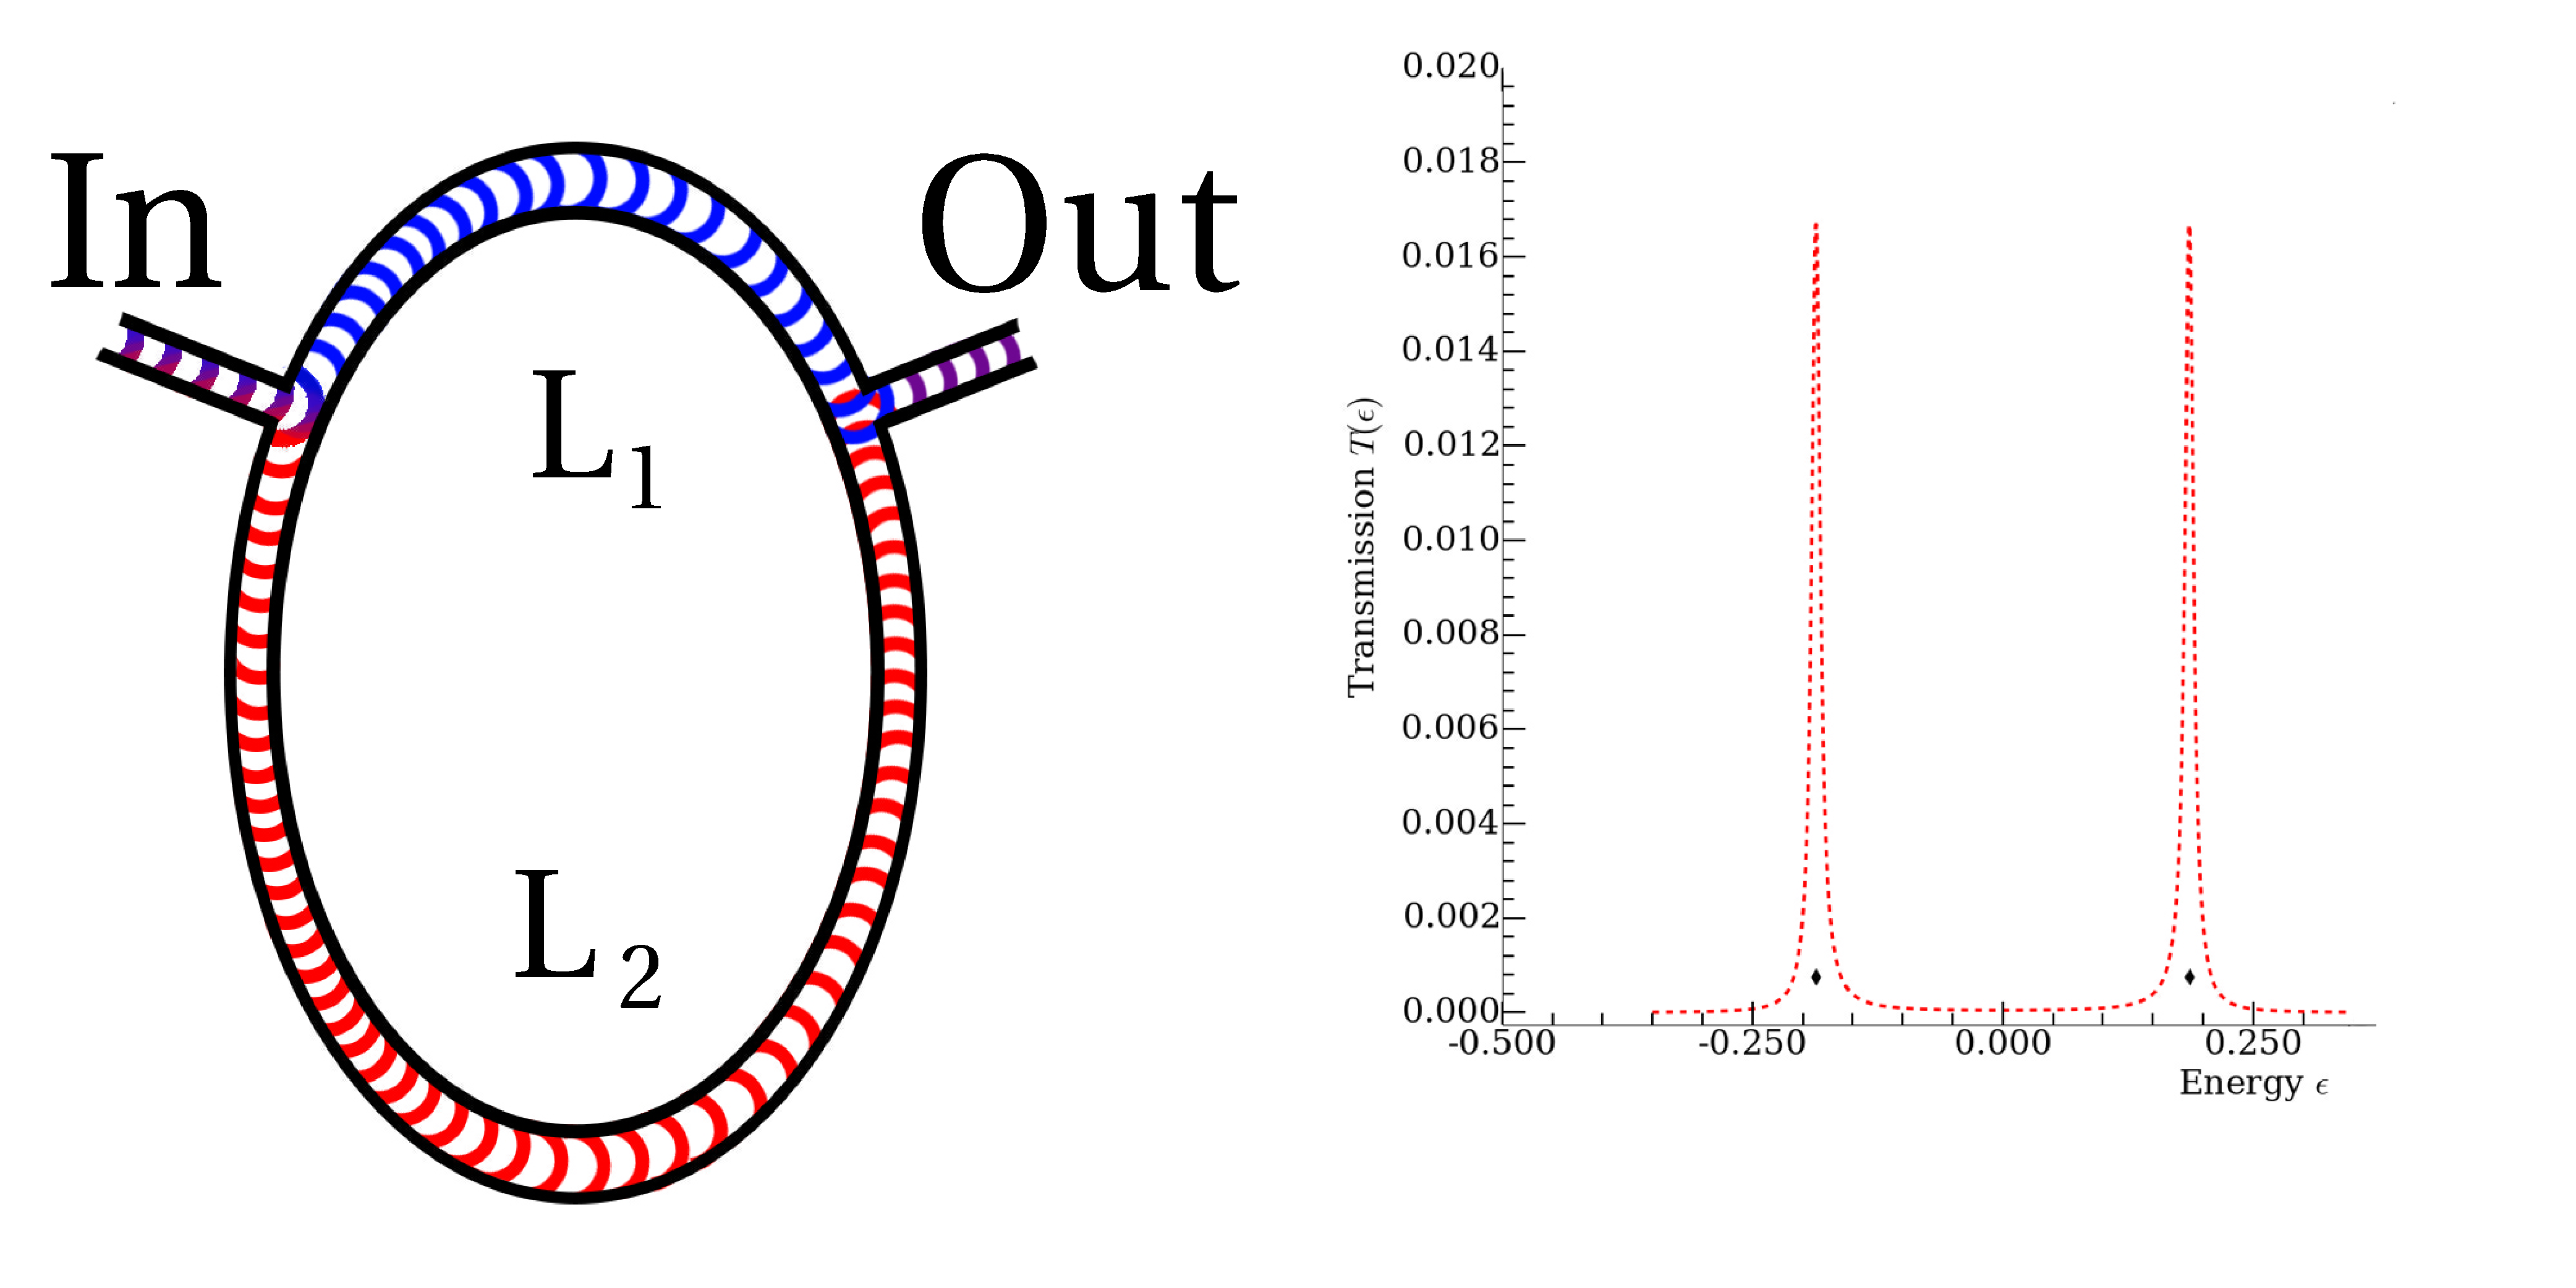
\includegraphics[height=0.5\textheight]{fig/acoustic.pdf}
        \caption{(left) Illustration of a instrument that would use interference. To the right, the notes or transmission peaks are shown.}
    \end{figure} 
\end{frame}%
\begin{frame}
    \frametitle{A music instrument.}
    \begin{figure}[!b] 
        \centering
        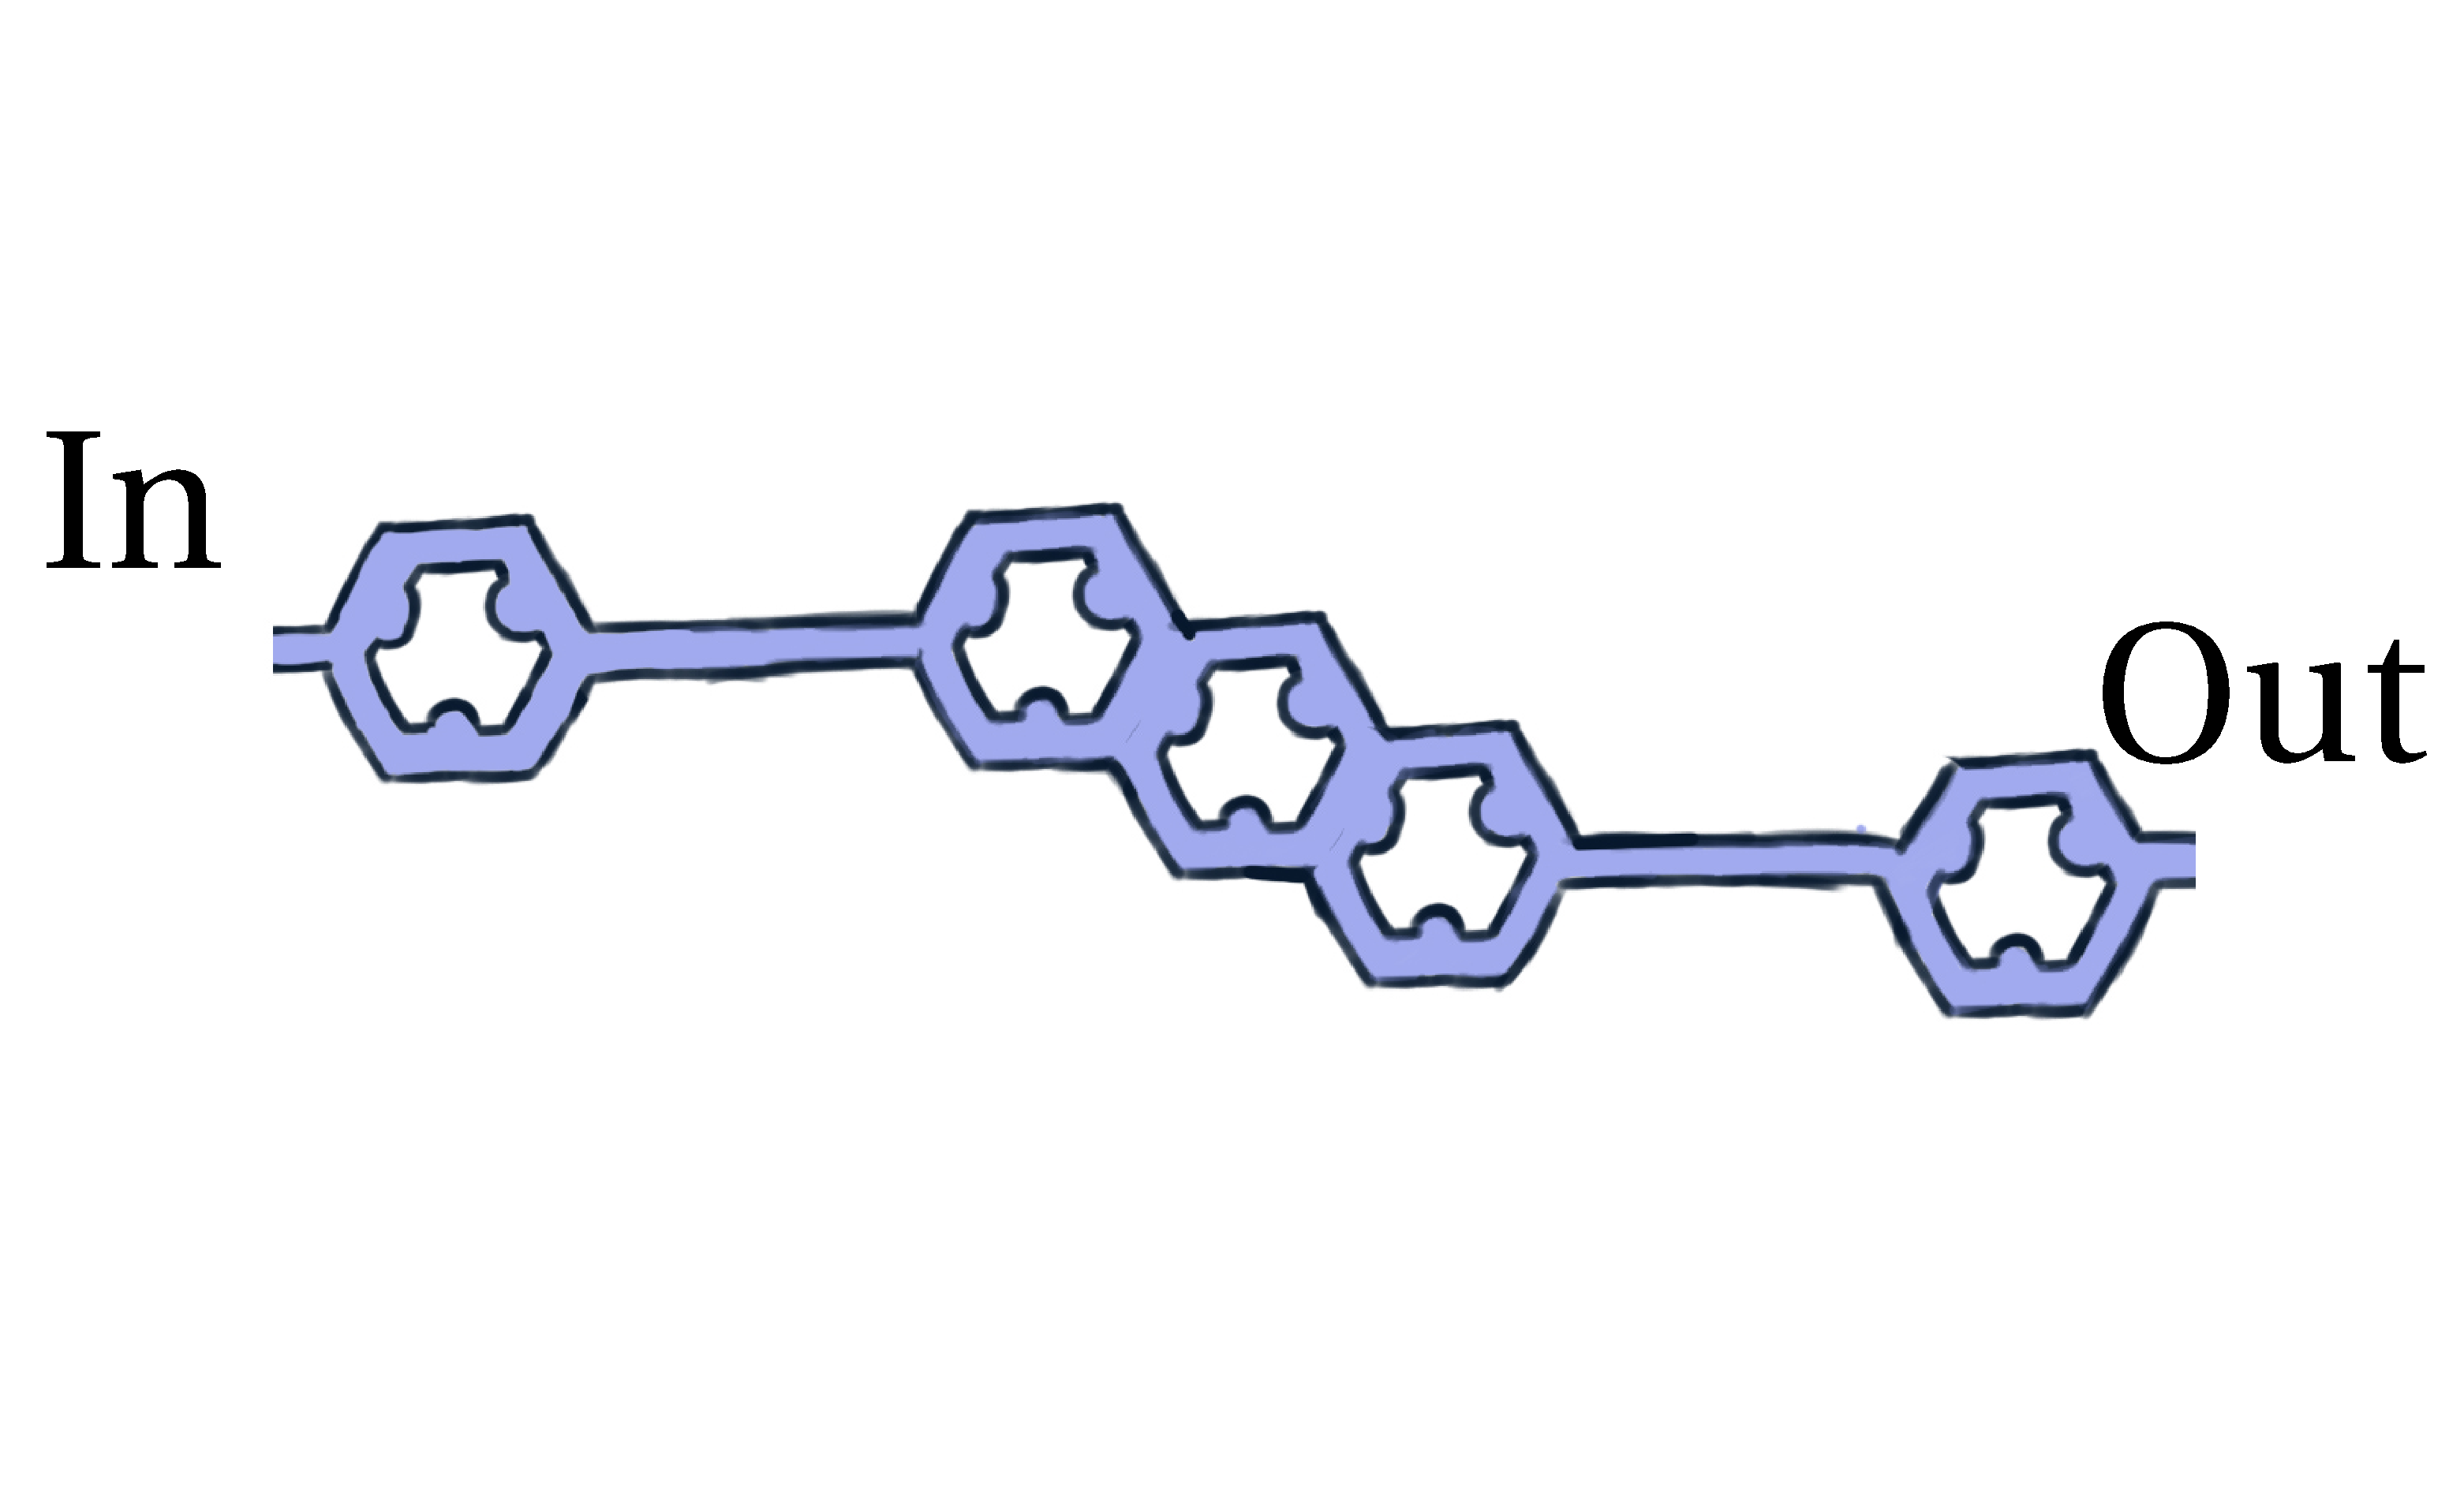
\includegraphics[height=0.5\textheight]{fig/molecule.pdf}
        \caption{The molecule displayed as a set of pipes to blow air through. Very complex, with many parts and lots of intersections.}
    \end{figure} 
\end{frame}%
\begin{frame}
    \frametitle{Flowing currents.}
    \begin{figure}[!b] 
        \centering
        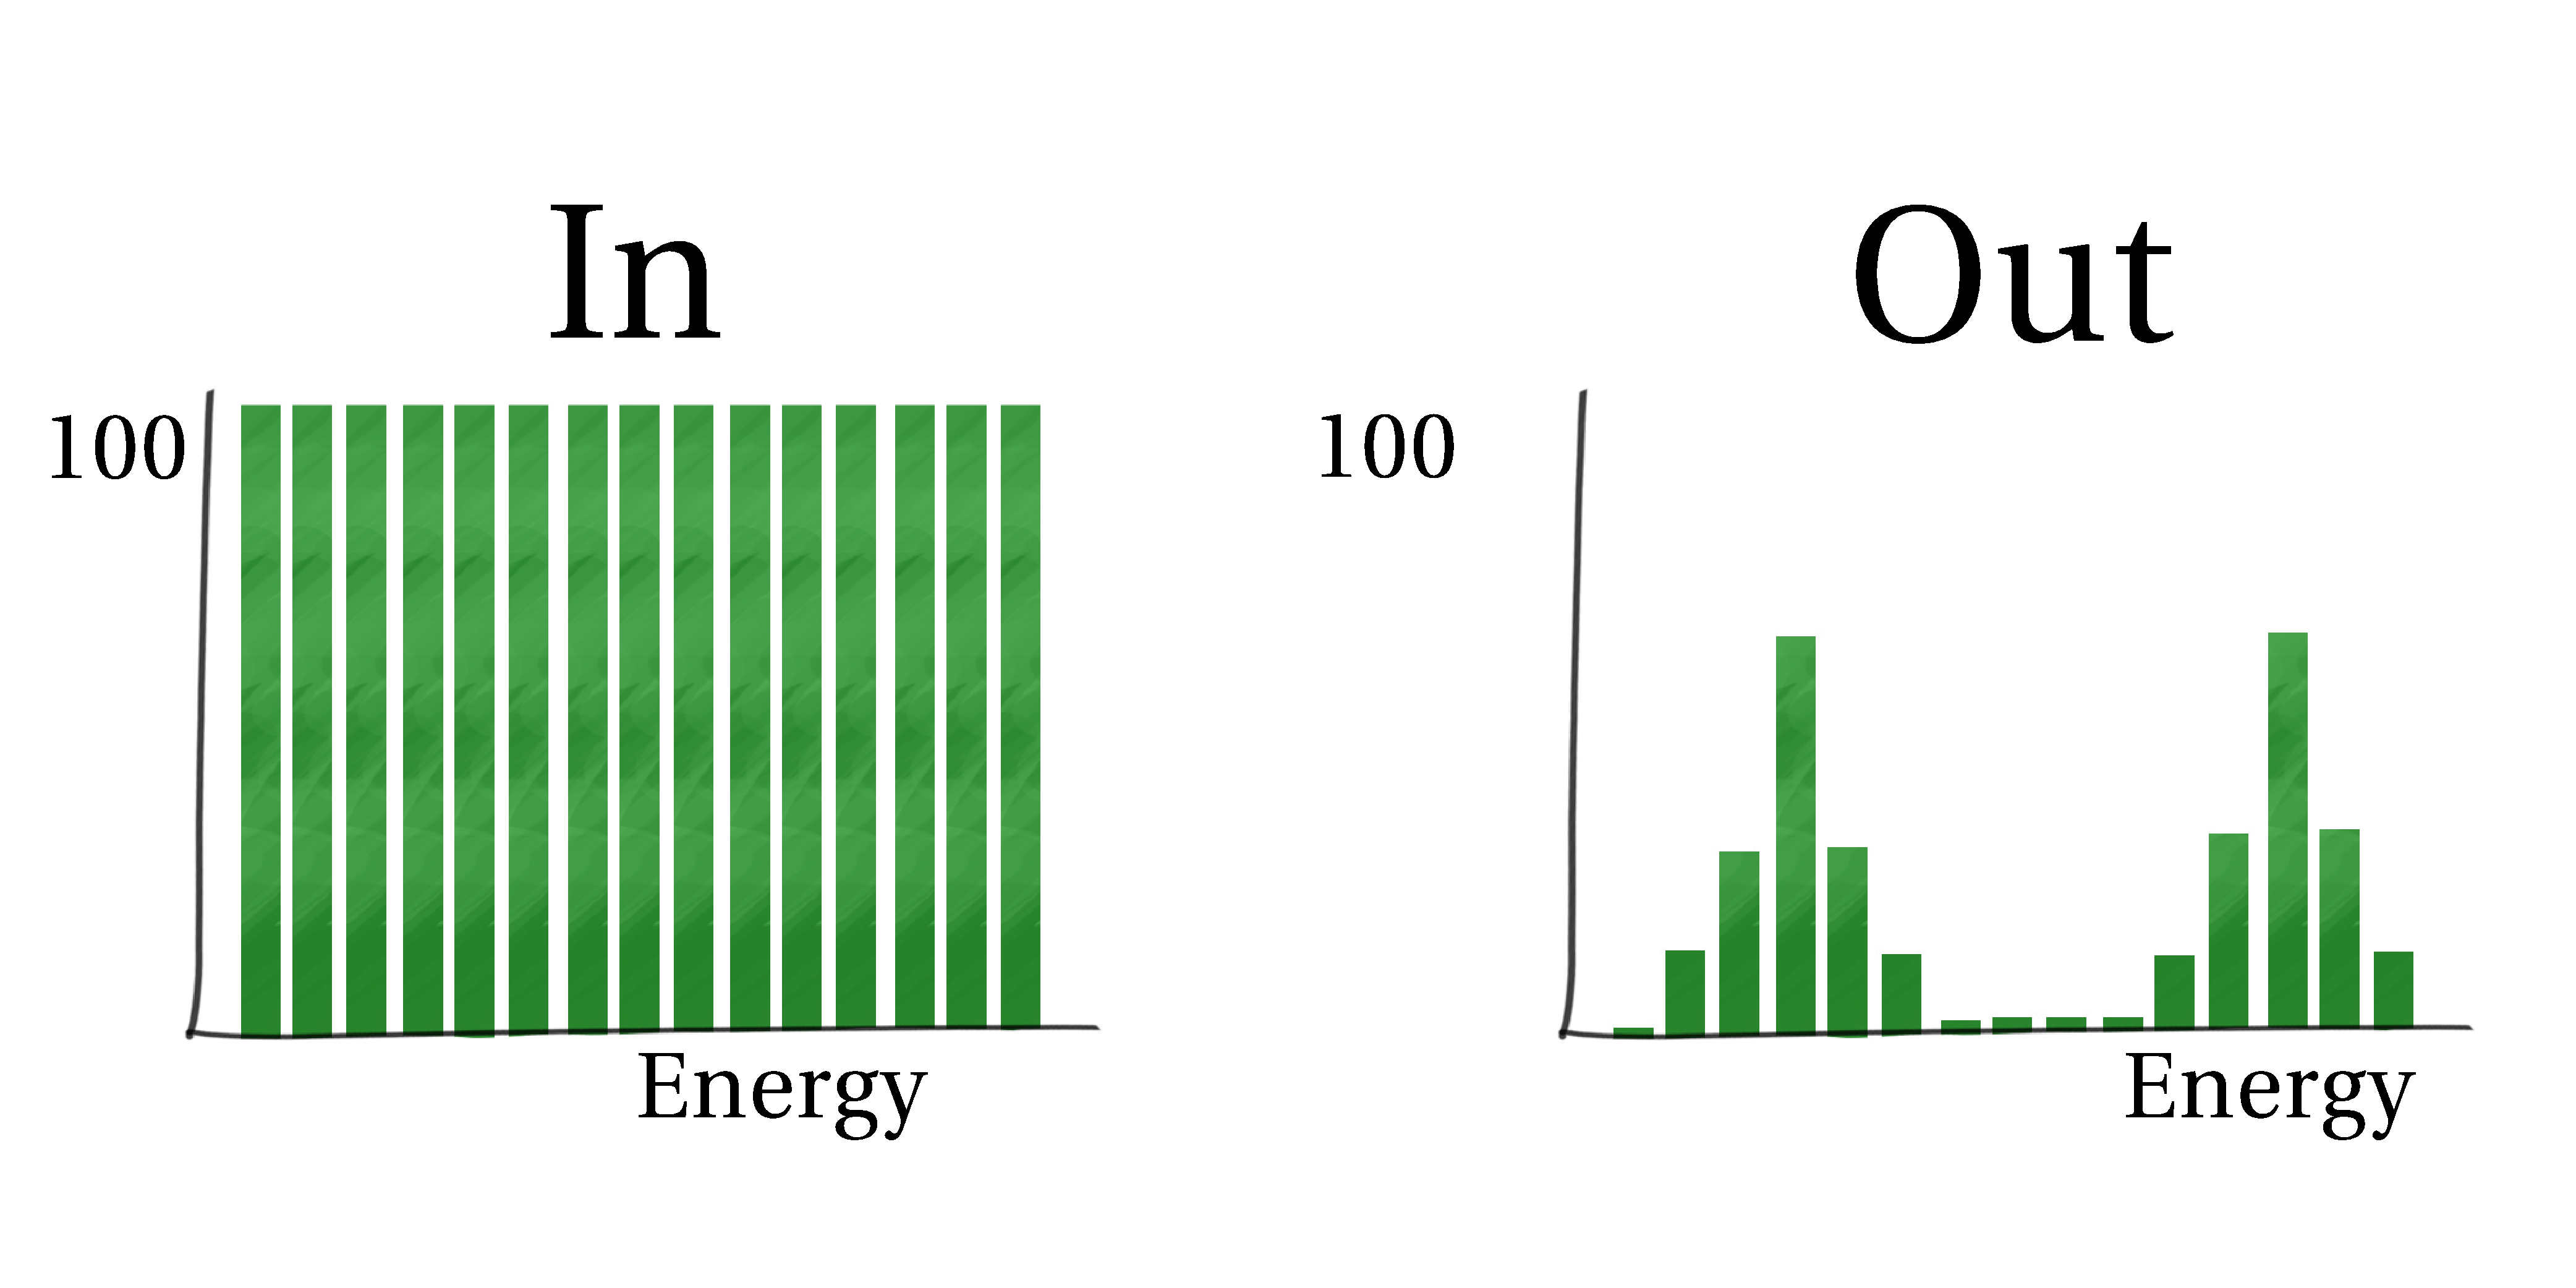
\includegraphics[height=0.5\textheight]{fig/current.pdf}
        \caption{To the left, we see the input-electrons, distributed at low-temperature. The right shows the electrons that pass the molecule - only those at the correct values.}
    \end{figure} 
\end{frame}%
\begin{frame}
    \frametitle{Current versus potential difference.}
    \begin{figure}[!b] 
        \centering
        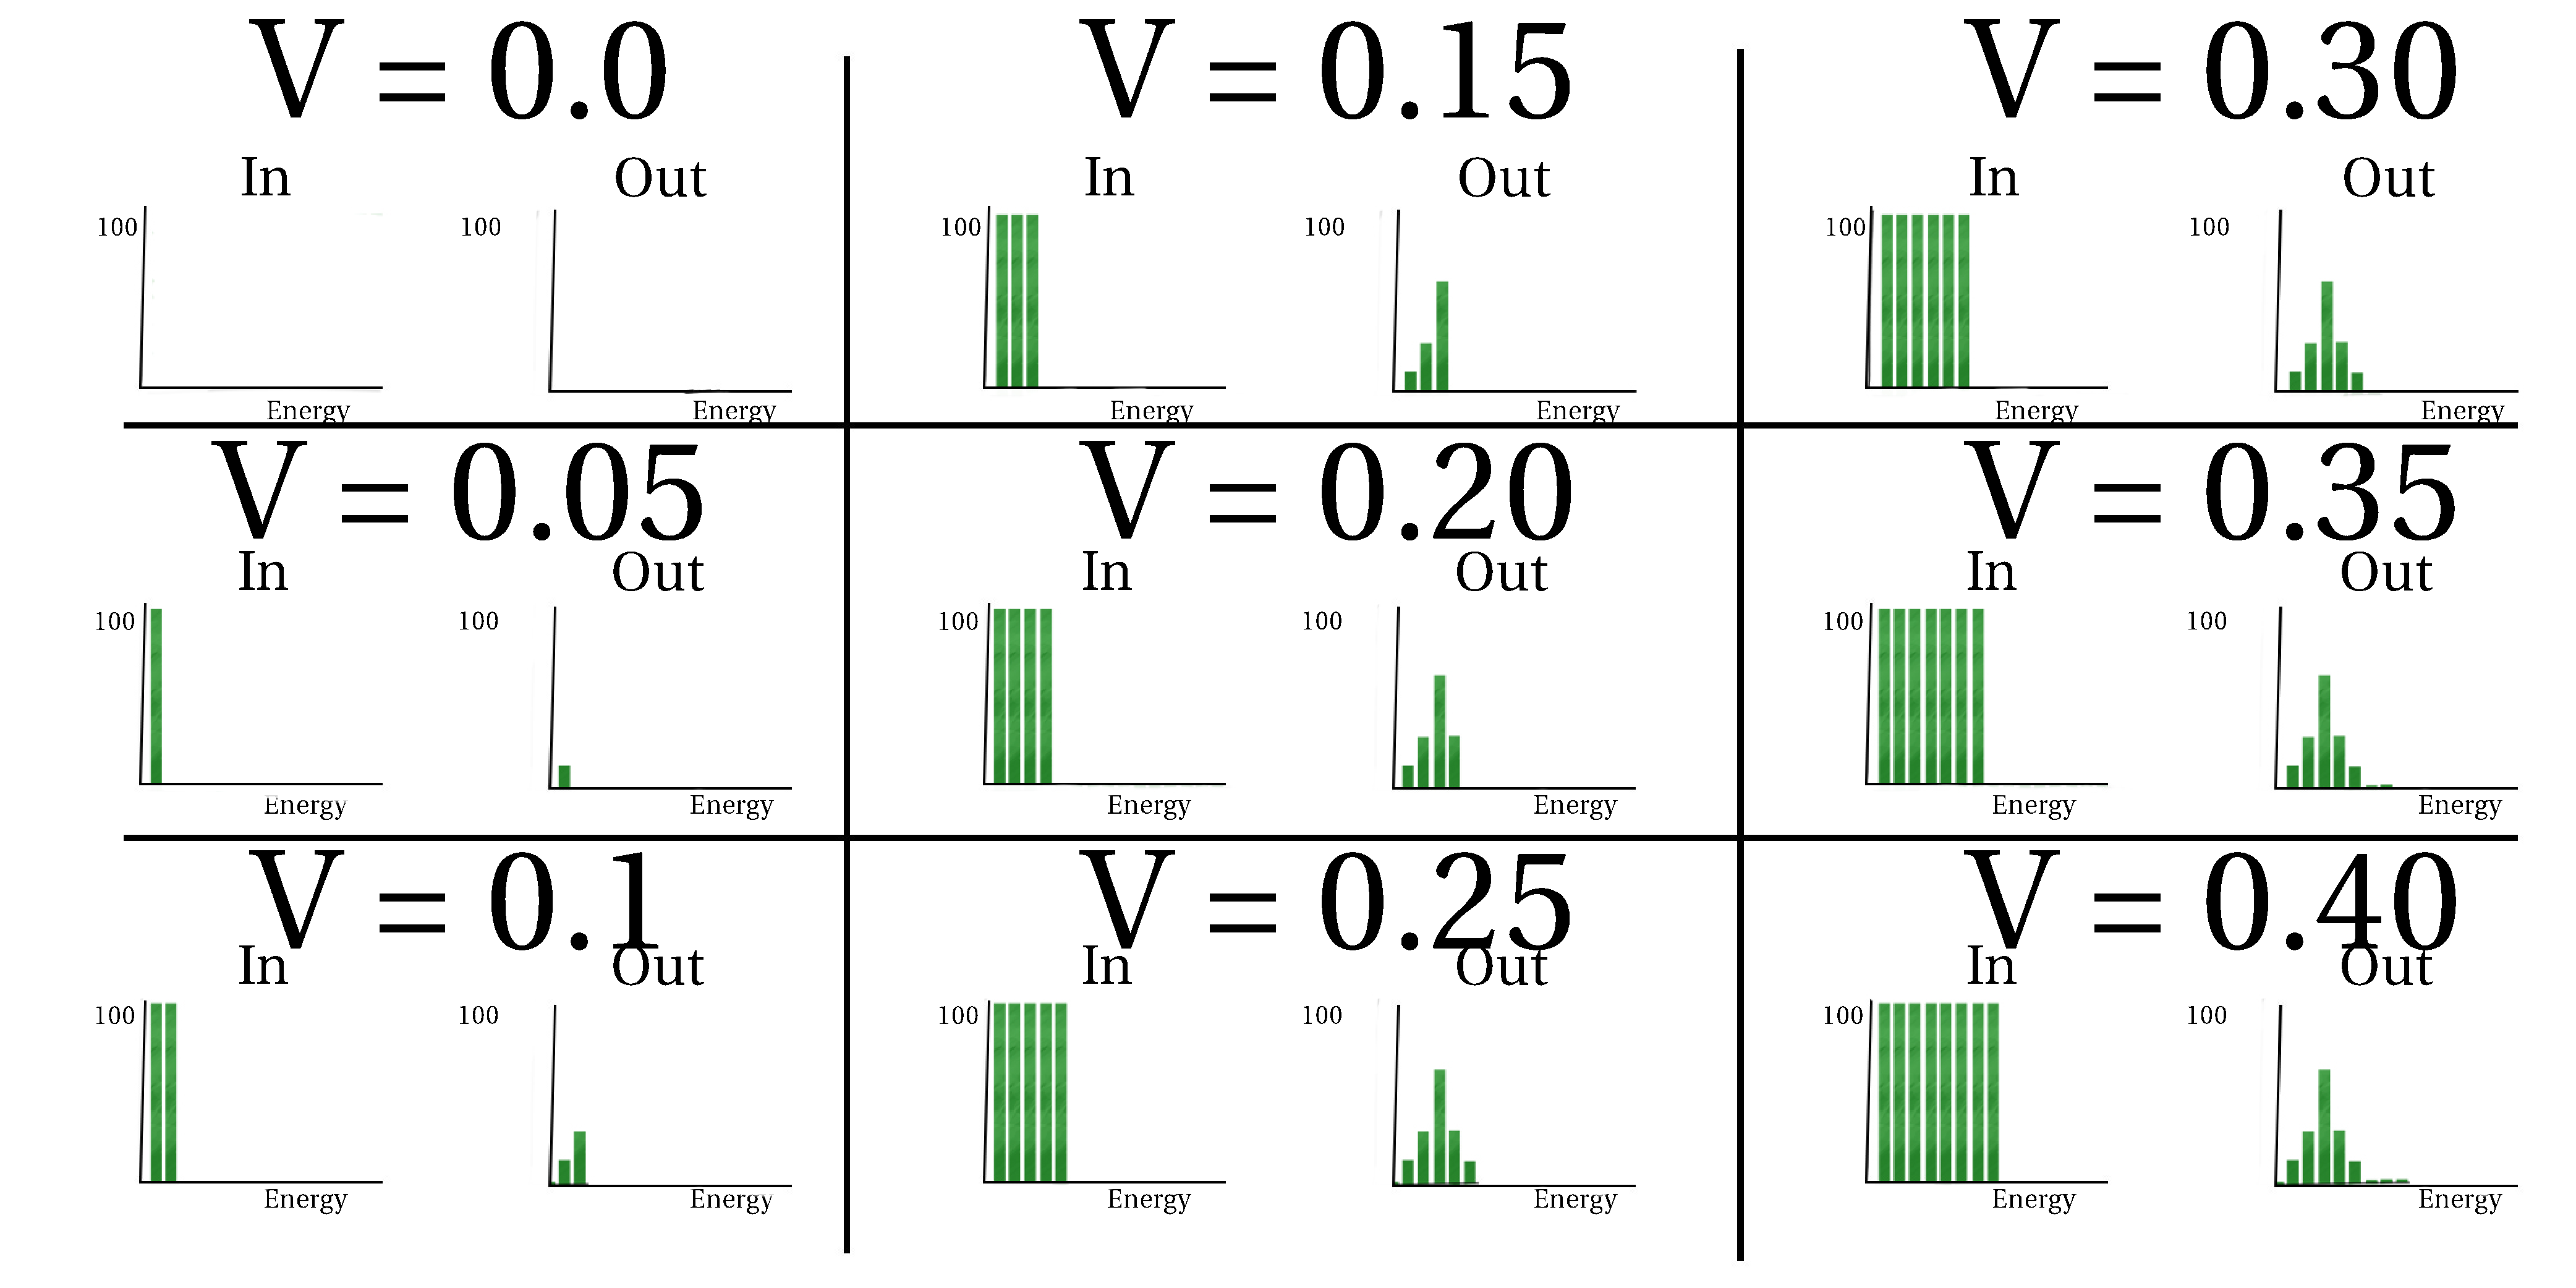
\includegraphics[width=\textwidth]{fig/current_calculation2.pdf}
        \caption{Image from the previous slide for various voltages.}
    \end{figure} 
\end{frame}%
\ssection{Summary}% 
\begin{frame}
    \frametitle{Summary.}
    \begin{itemize}
        \item Molecules are complicated.
        \item Molecules have 'notes' or so-called \emph{transmission peaks}.
        \item The \emph{Green's Function formalism} can calculate the transmission peaks.
        \item The transmission peaks determine the \emph{current}.
        \item The current is found by putting blocks of electrons through the transmission graph, and counting how many came out.
        \item Various things haven't been calculated yet.
    \end{itemize} 
\end{frame}%
\begin{frame}
    \frametitle{Next}
	\tableofcontents[currentsection,currentsubsection]
\end{frame}
\section{Theory}
\ssection{Green's Functions}
\begin{frame}
    \frametitle{The Single-Particle Green's Function}
     \begin{itemize}
     \item A particle is created in state $i$ at time $t'$.
     \item The Green's function $G_{ij}(t,t')$.
     \item The probability it is found in state $j$ at time $t$.
     \item Green's Function contains the sum of all possible interactions
     \end{itemize}
    
    \begin{figure}[!b] 
        \centering
        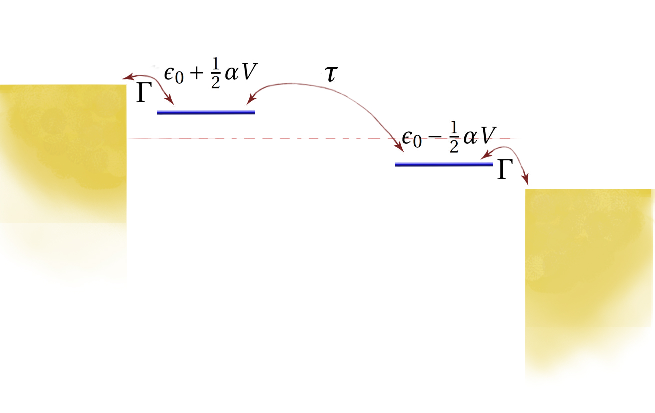
\includegraphics[height=0.5\textheight]{fig/non_interacting_schematics.pdf}
        \caption{Single-Particle Green's Function in a picture.}
    \end{figure} 
\end{frame} 
\begin{frame}
    \frametitle{Coulomb Interaction}
     \begin{itemize}
     \item Electrons carry charge $-e$.
     \item Electrons repulse.
     \item Interaction energy $U = \braket{\varphi_1 \left| V(r^\mu_1, r^\mu_2)\right|\varphi_2}$.
     \item Add to Green's Function?
     \end{itemize}
    
    \begin{figure}[!b] 
        \centering
        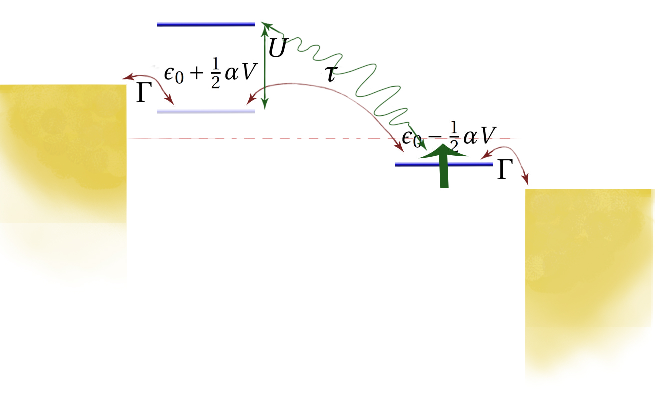
\includegraphics[height=0.5\textheight]{fig/interacting_schematics.pdf}
        \caption{Single-Particle Green's Function in a picture.}
    \end{figure} 
\end{frame}
\begin{frame}
    \frametitle{Many-Body Green's Function} 
    Denoted $\mathscr{G}(\epsilon)$.
    \begin{figure}[!b]  
        \begin{subfigure}{0.45\textwidth}\centering
            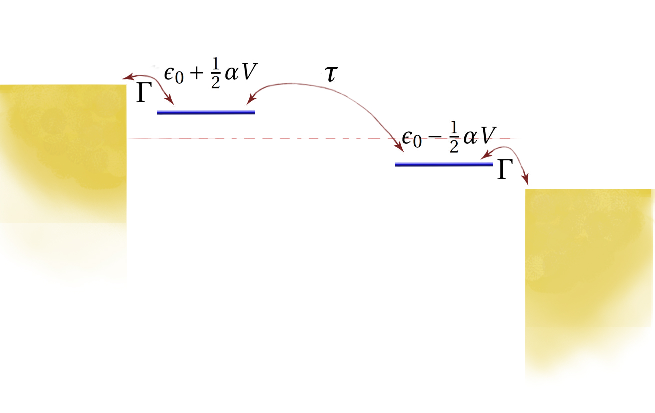
\includegraphics[clip=true,trim=0cm 1cm 0cm 0cm, width=0.65\textwidth]{fig/non_interacting_schematics.pdf}
            \caption{No electrons present.}
        \end{subfigure}~ 
        \begin{subfigure}{0.45\textwidth}\centering
            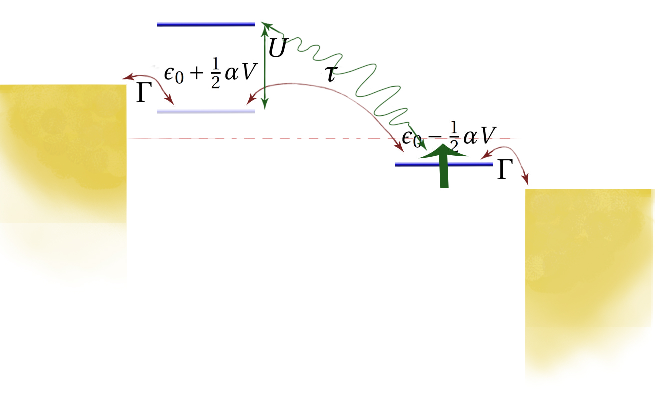
\includegraphics[clip=true,trim=0cm 1cm 0cm 0cm, width=0.65\textwidth]{fig/interacting_schematics.pdf}
            \caption{Electron present on the right.}
        \end{subfigure}
        
         
        \begin{subfigure}{0.45\textwidth}\centering
            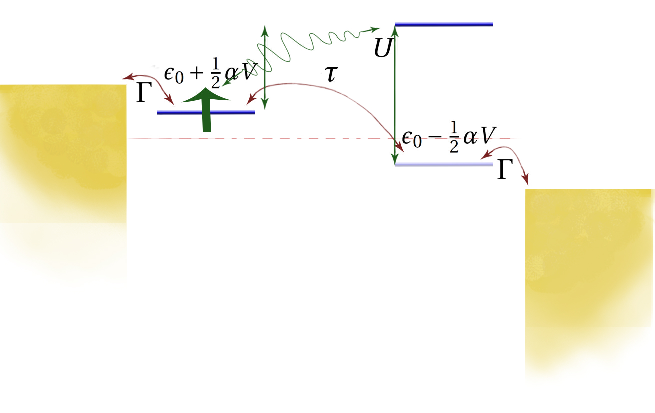
\includegraphics[clip=true,trim=0cm 1cm 0cm 0cm, width=0.65\textwidth]{fig/interacting_schematics2.pdf}
            \caption{Electron present on the left.}
        \end{subfigure}~ 
        \begin{subfigure}{0.45\textwidth}\centering
            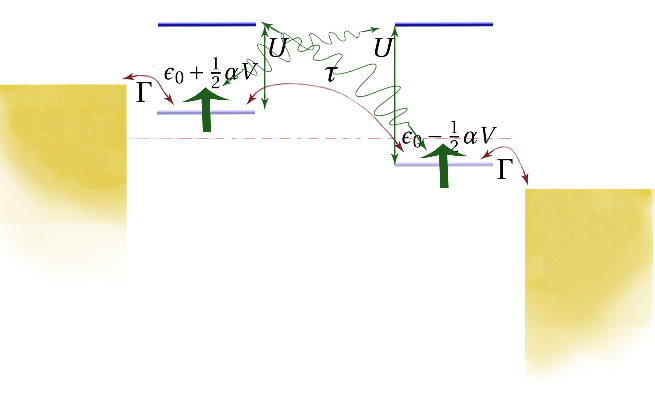
\includegraphics[clip=true,trim=0cm 1cm 0cm 0cm, width=0.75\textwidth]{fig/interacting_schematics3.pdf}
            \caption{Electron present on both the right and the left.}
        \end{subfigure}
        \caption{The many-body Green's Function is found as a weighted sum of single-particle Green's Functions.} 
    \end{figure} 
\end{frame} 
\ssection{Density Matrix}
\begin{frame}
    \frametitle{Density Matrix}
    \begin{itemize}
        \item What are the chances for each of the pictures? (many-body states)
        \item Mathematically, chance is defined as $P_{\lambda}$, e.g. $P_{01}$ for the state with one electron on the right level.
        \item In equilibrium, the energy of each state determines the chance.
        \item At low temperature, the state with the lowest energy is occupied.
        \item Boltzmann $P_\lambda = Z^{-1} \text{exp}\left\{ - \frac{E_\lambda}{k_b T}\right\}$, $Z$ normalisation constant called the partition function.
        \item However... The molecule is inside the potential difference, and is not in equilibrium.
        \item What now?
    \end{itemize} 
\end{frame}%
\begin{frame}
    \frametitle{Non-equilibrium Density Matrix}
    \begin{itemize}
        \item Suppose $P_\lambda$ is known for all $\lambda$.
        \item The states with one electron on the right level are $P_{01}, P_{11}$.
        \item The expected number of electrons on the right level is $\braket{n_R} = 1 \times P_{01} + 1 \times P_{11}$.
        \item Matrix notation: \begin{align*}\braket{ \begin{pmatrix} n_L \\ n_R \end{pmatrix}} = \begin{pmatrix} 0 & 0 & 1 & 1 \\ 0 & 1 & 0 & 1\end{pmatrix}\begin{pmatrix} P_{00} \\ P_{01} \\ P_{10} \\ P_{11} \end{pmatrix}\end{align*}
        \item Left-Hand side can also be found from Green's function $\mathscr{G}^{<}$. (Complicated expression). Requires the vector of probabilities.
    \end{itemize} 
\end{frame}%
\begin{frame}
    \frametitle{Self-consistent Density Matrix}
    \begin{itemize} 
    \item Required: vector of probabilities $\underline{P}$
    \item $\braket{\underline{n}}$ can be found in two ways.
    \item $\braket{\underline{n}} = K P$ from the last slide.
    \item $\braket{\underline{n}} = W(\underline{P})$ via the lesser Green's function $\mathscr{G}^<$. 
    \item Use a self-consistent scheme to find $\underline{P}$!
    \item Given some value of $\underline{P}$, find $W(\underline{P}) = \braket{W}$.
    \item Solve $ K \underline{P} = \braket{W}$ for P.
    \item However, matrix $K$ is not square. Use minimisation?
    \end{itemize} 
\end{frame}%
\begin{frame}
    \frametitle{Self-consistent scheme}
    \begin{enumerate} 
    \item Initial guess $\underline{P}^0$ as equilibrium (Boltzmann).
    \item Calculate $W(\underline{P}^0) = \braket{W}^0$.
    \item Minimise $K \underline{P}^1 = \braket{W}^0$ to find the next-generation $P$.
    \item Check if $P^1 = P^0$. If not, return to step 2. Else...
    \item You have found the non-equilibrium $\underline{P}$, which just so happens to be the diagonal of the density-matrix $\braket{\rho}$.
    \end{enumerate} 
    
    Sounds simple. However, takes extremely long to reach step 5. 
    
    Because $T\approx 6$K, I have approximated the \emph{non}-equilibrium density matrix as a equilibrium density matrix. 
\end{frame}% 
\begin{frame}
    \frametitle{Next}
	\tableofcontents[currentsection,currentsubsection]
\end{frame}
\section{Results}
\ssection{Transmission}
\begin{frame}
    \frametitle{Transmission}
    \vspace{-3mm}
    \begin{figure}[!b] 
        \centering
        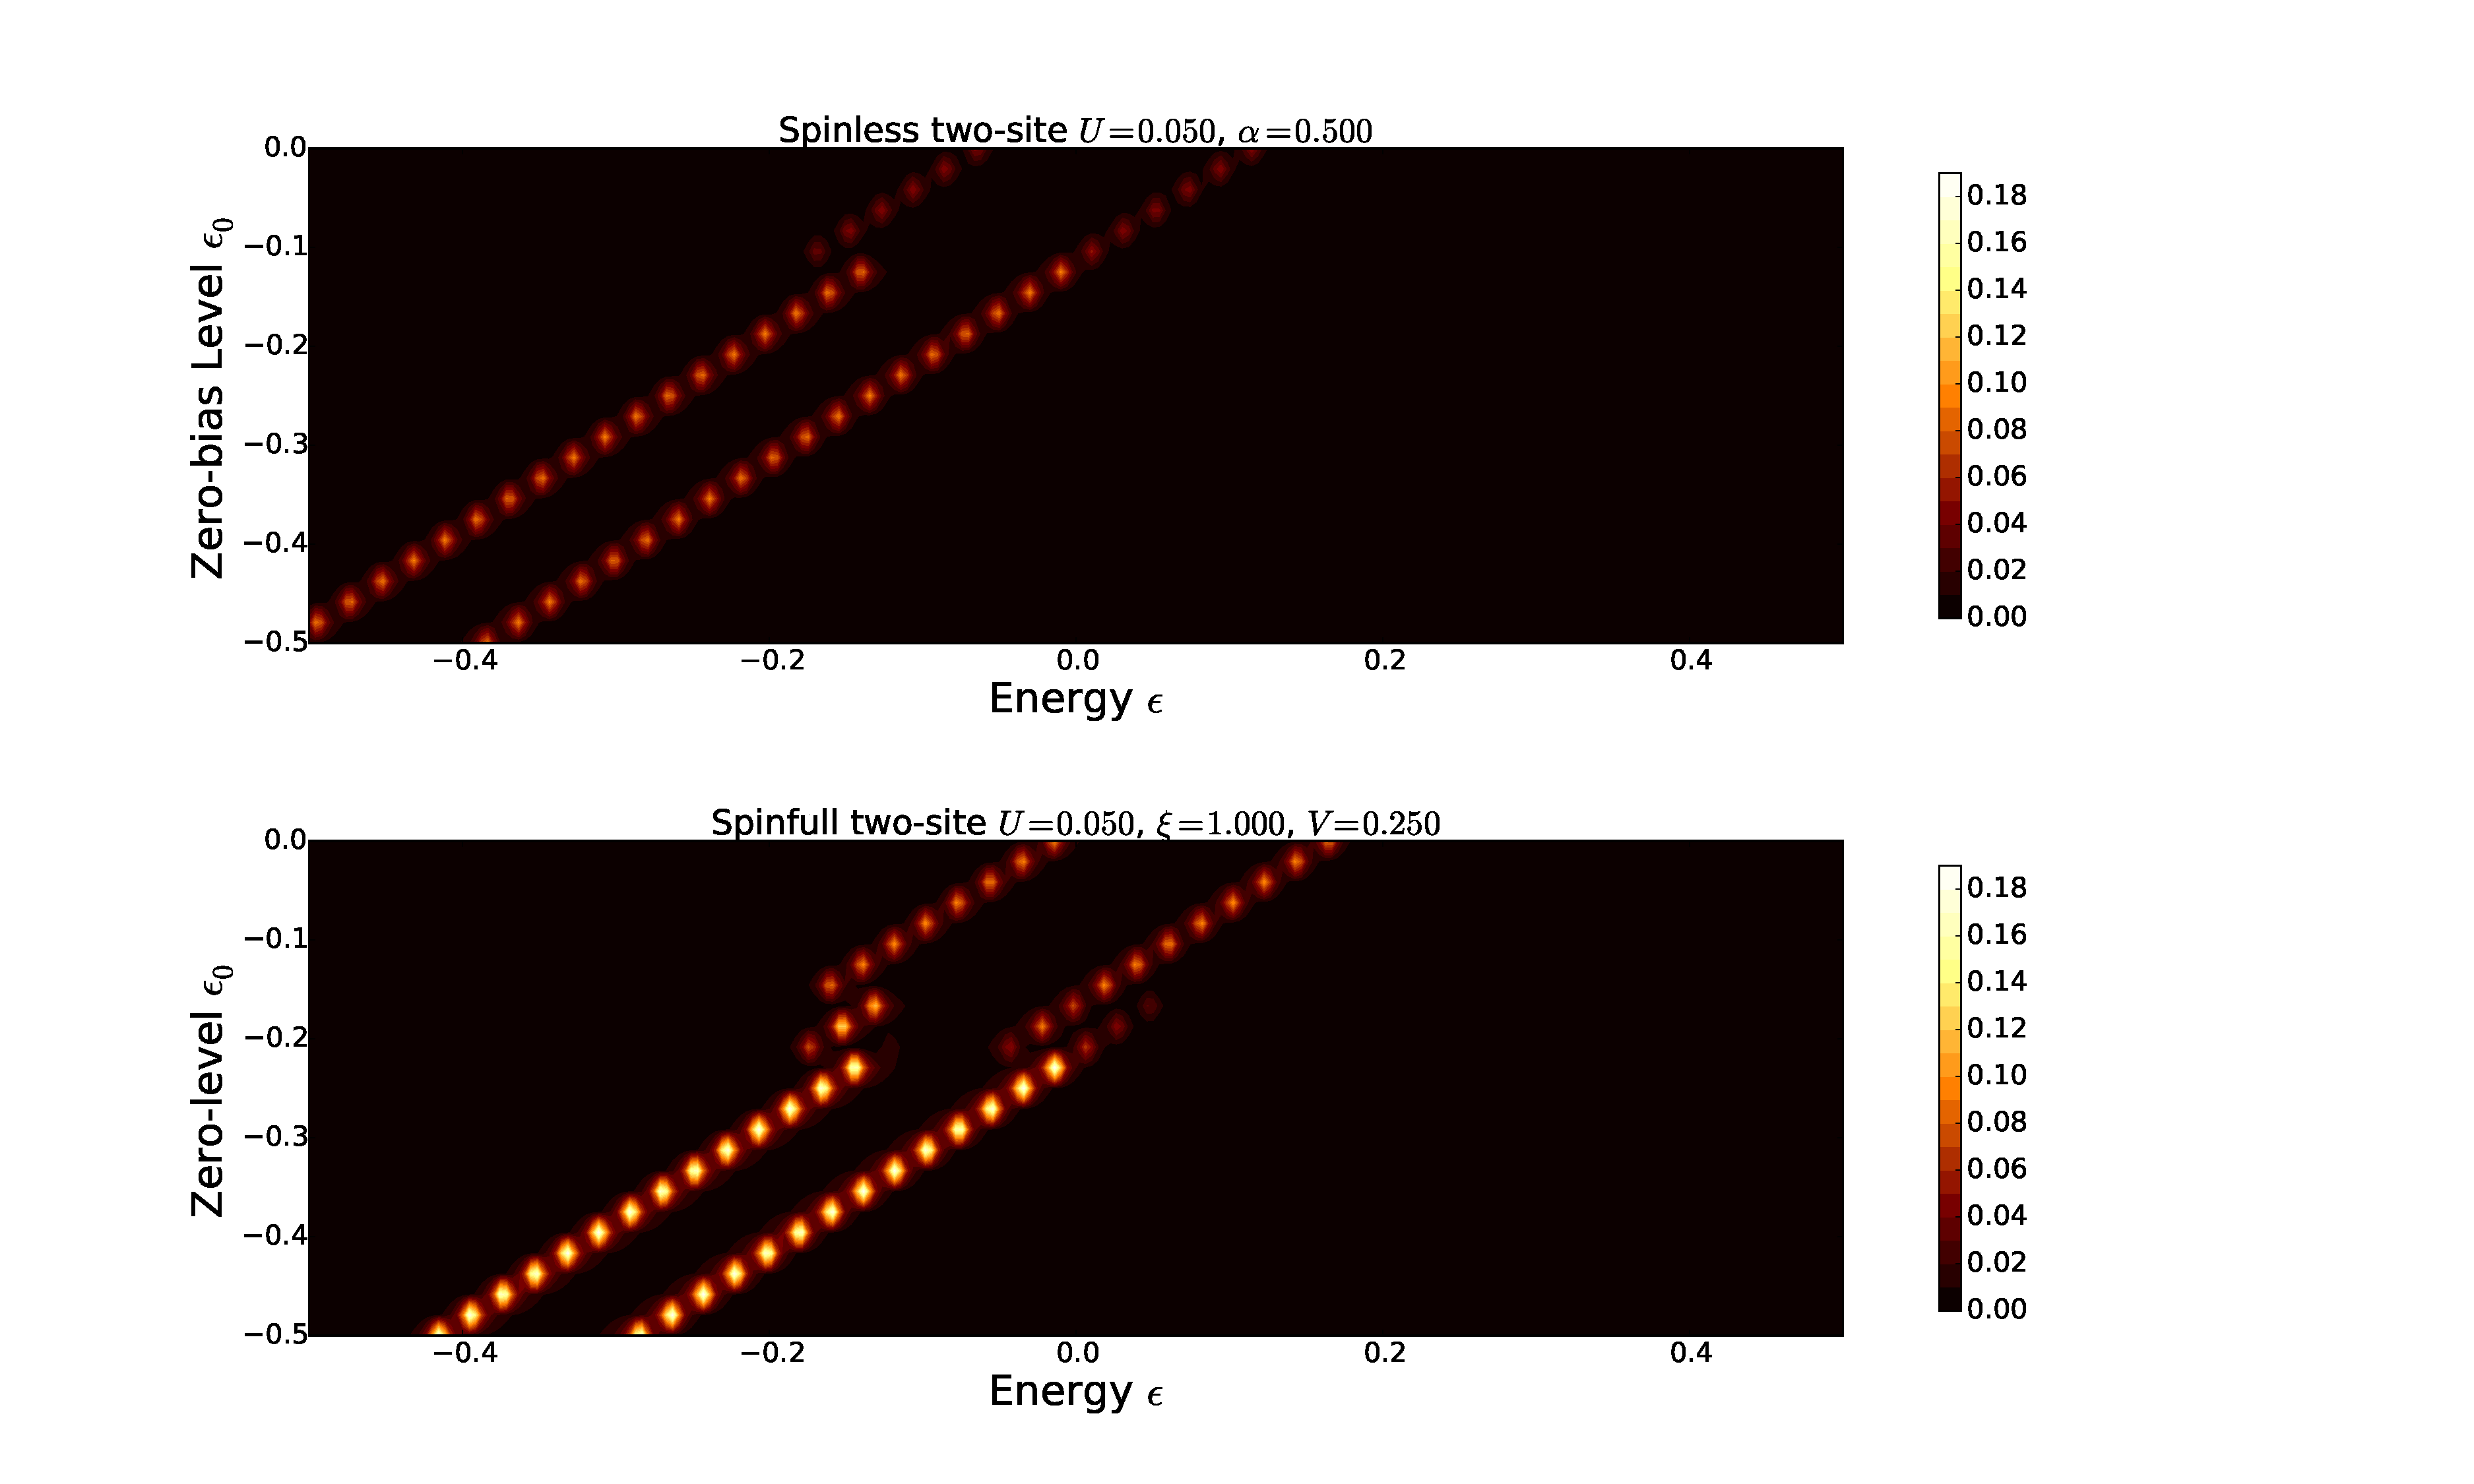
\includegraphics[height=.85\textheight, width=\textwidth,clip=true, trim=0cm 0cm 5cm 2cm]{res/transmap_u1_k2.pdf}
        \vspace{-6mm}
        \caption{Spinless versus Spinfull Transmission at certain parameters.}
    \end{figure} 
\end{frame}
\ssection{Coulomb Diamonds I}
\begin{frame}
    \frametitle{Coulomb Diamonds}
    \vspace{-3mm}
    \begin{figure}[!b] 
        \centering
        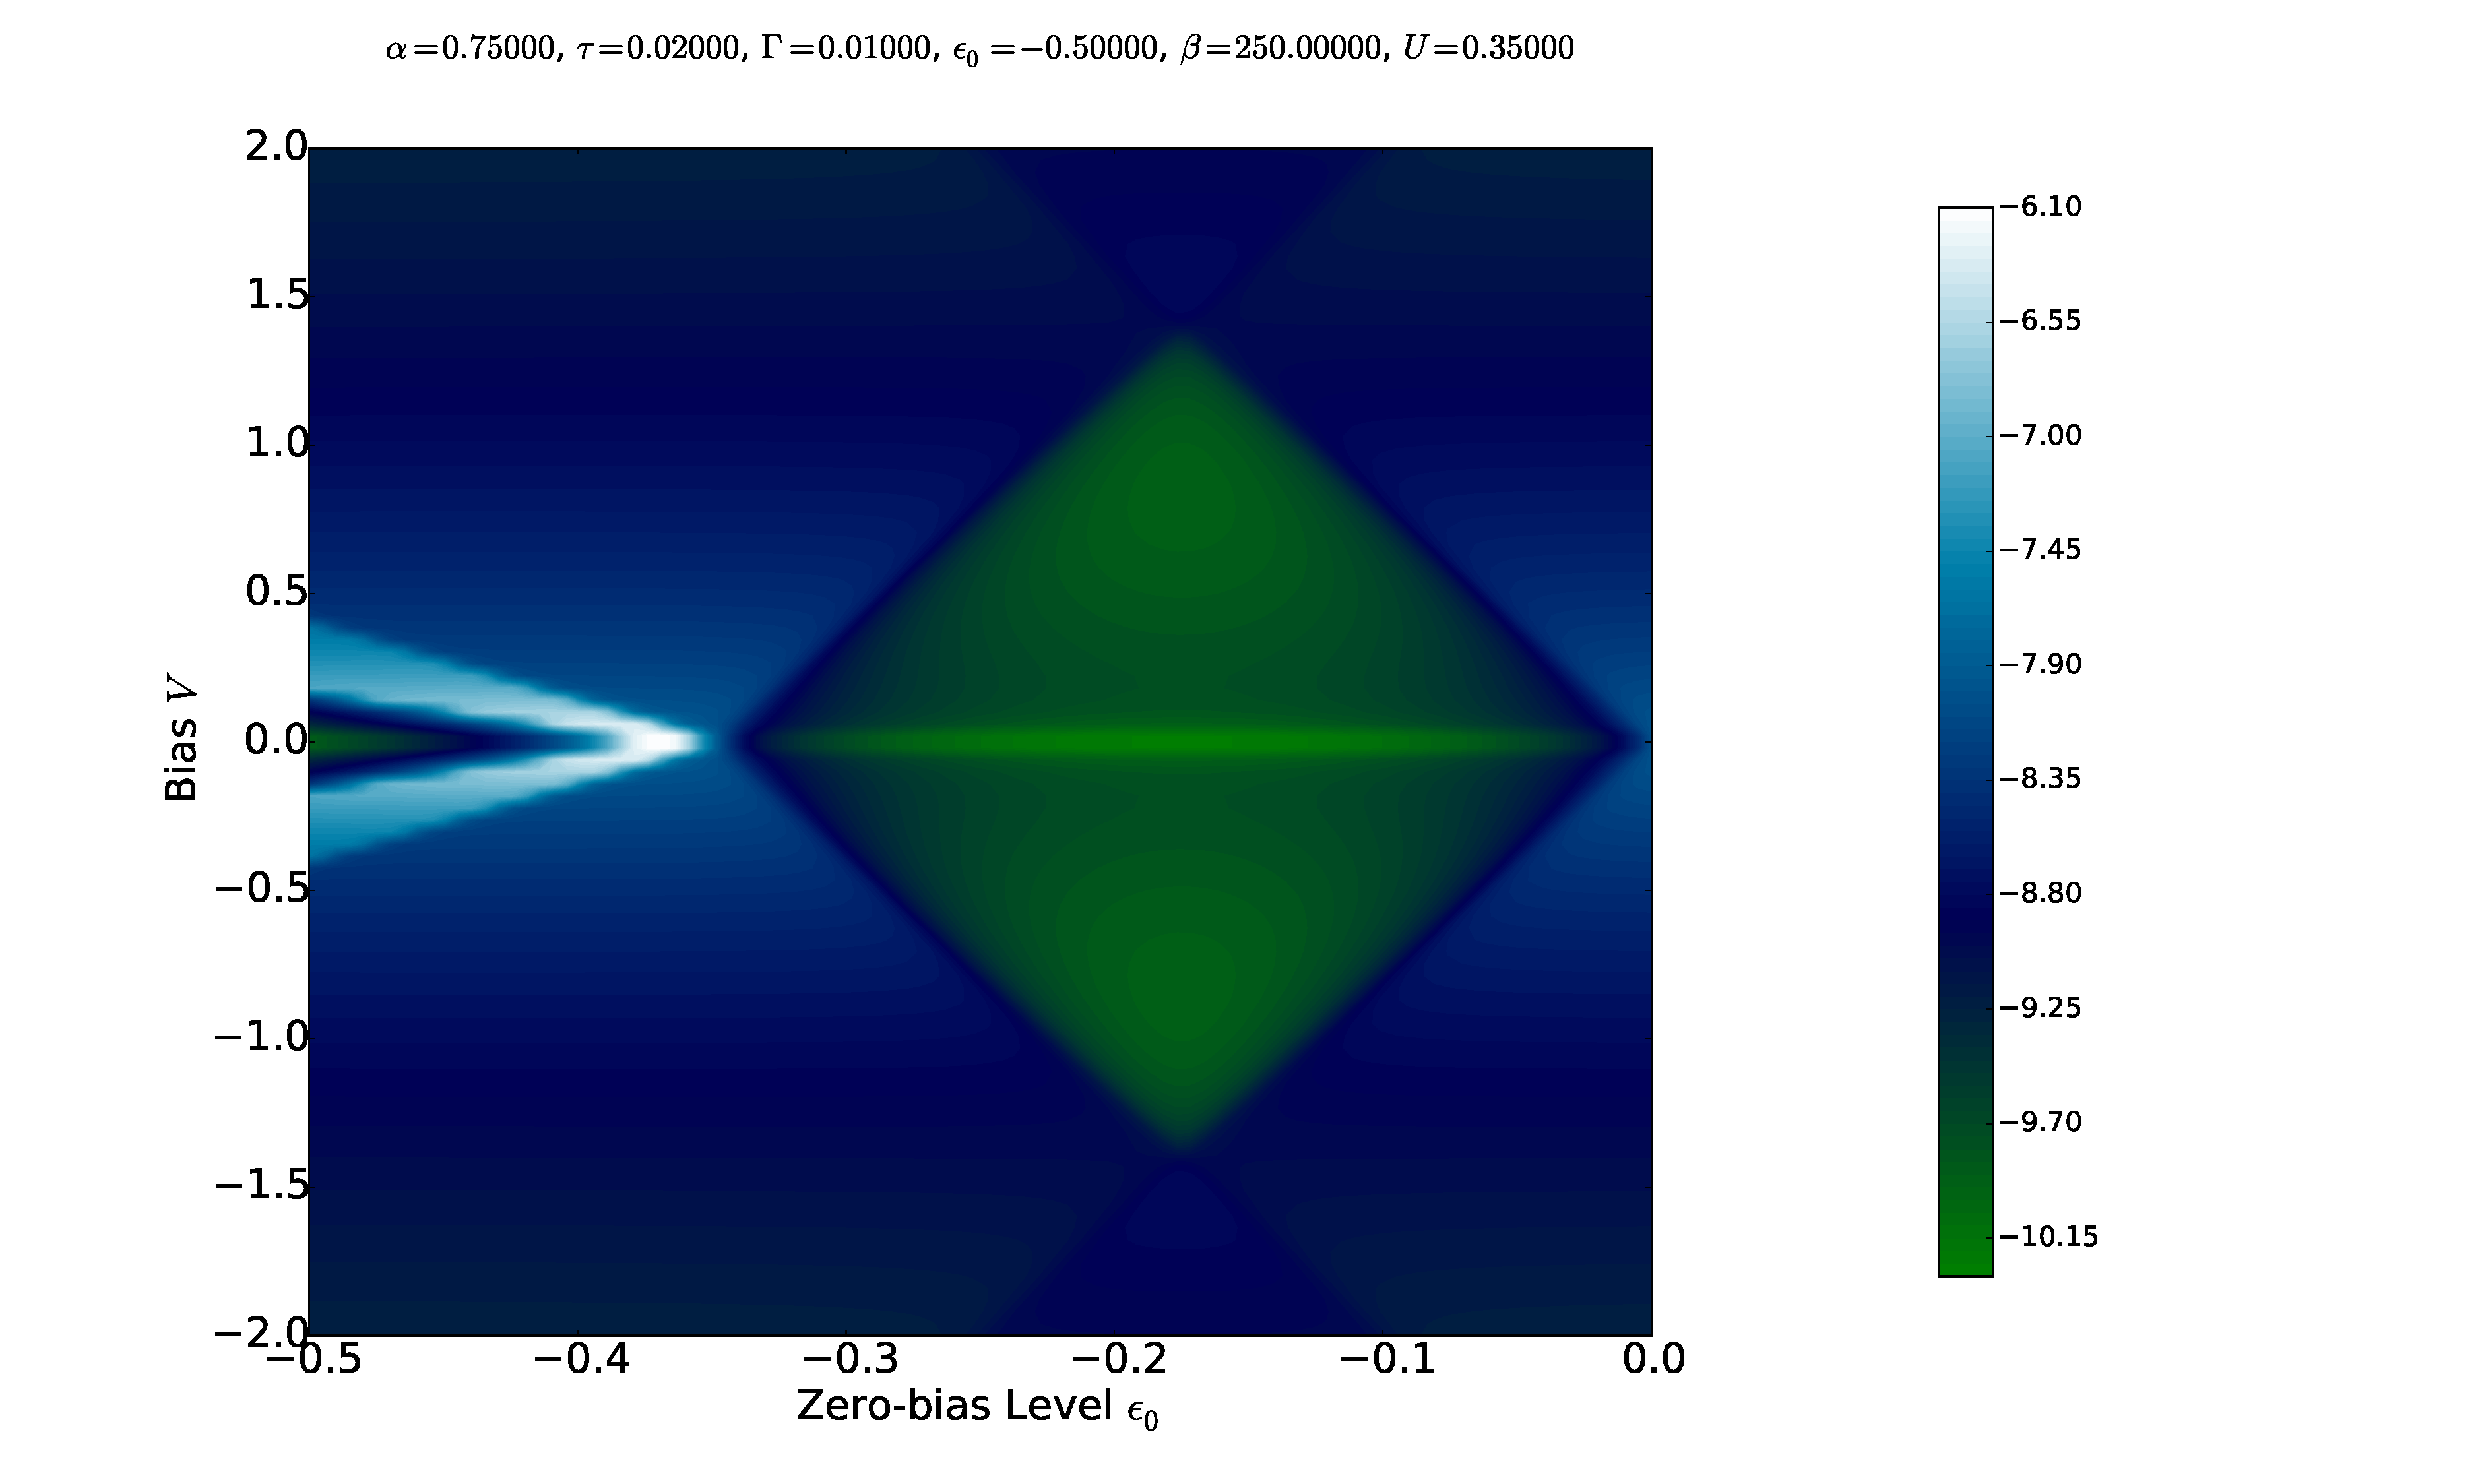
\includegraphics[height=.85\textheight, width=\textwidth]{res/current_map_diamond_alpha_075.pdf}
        \vspace{-6mm}
        \caption{Large Coulomb Diamond, width is $U$.}
    \end{figure} 
\end{frame}
\begin{frame}
    \frametitle{Coulomb Diamonds II}
    \vspace{-3mm}
    \begin{figure}[!b] 
        \centering
        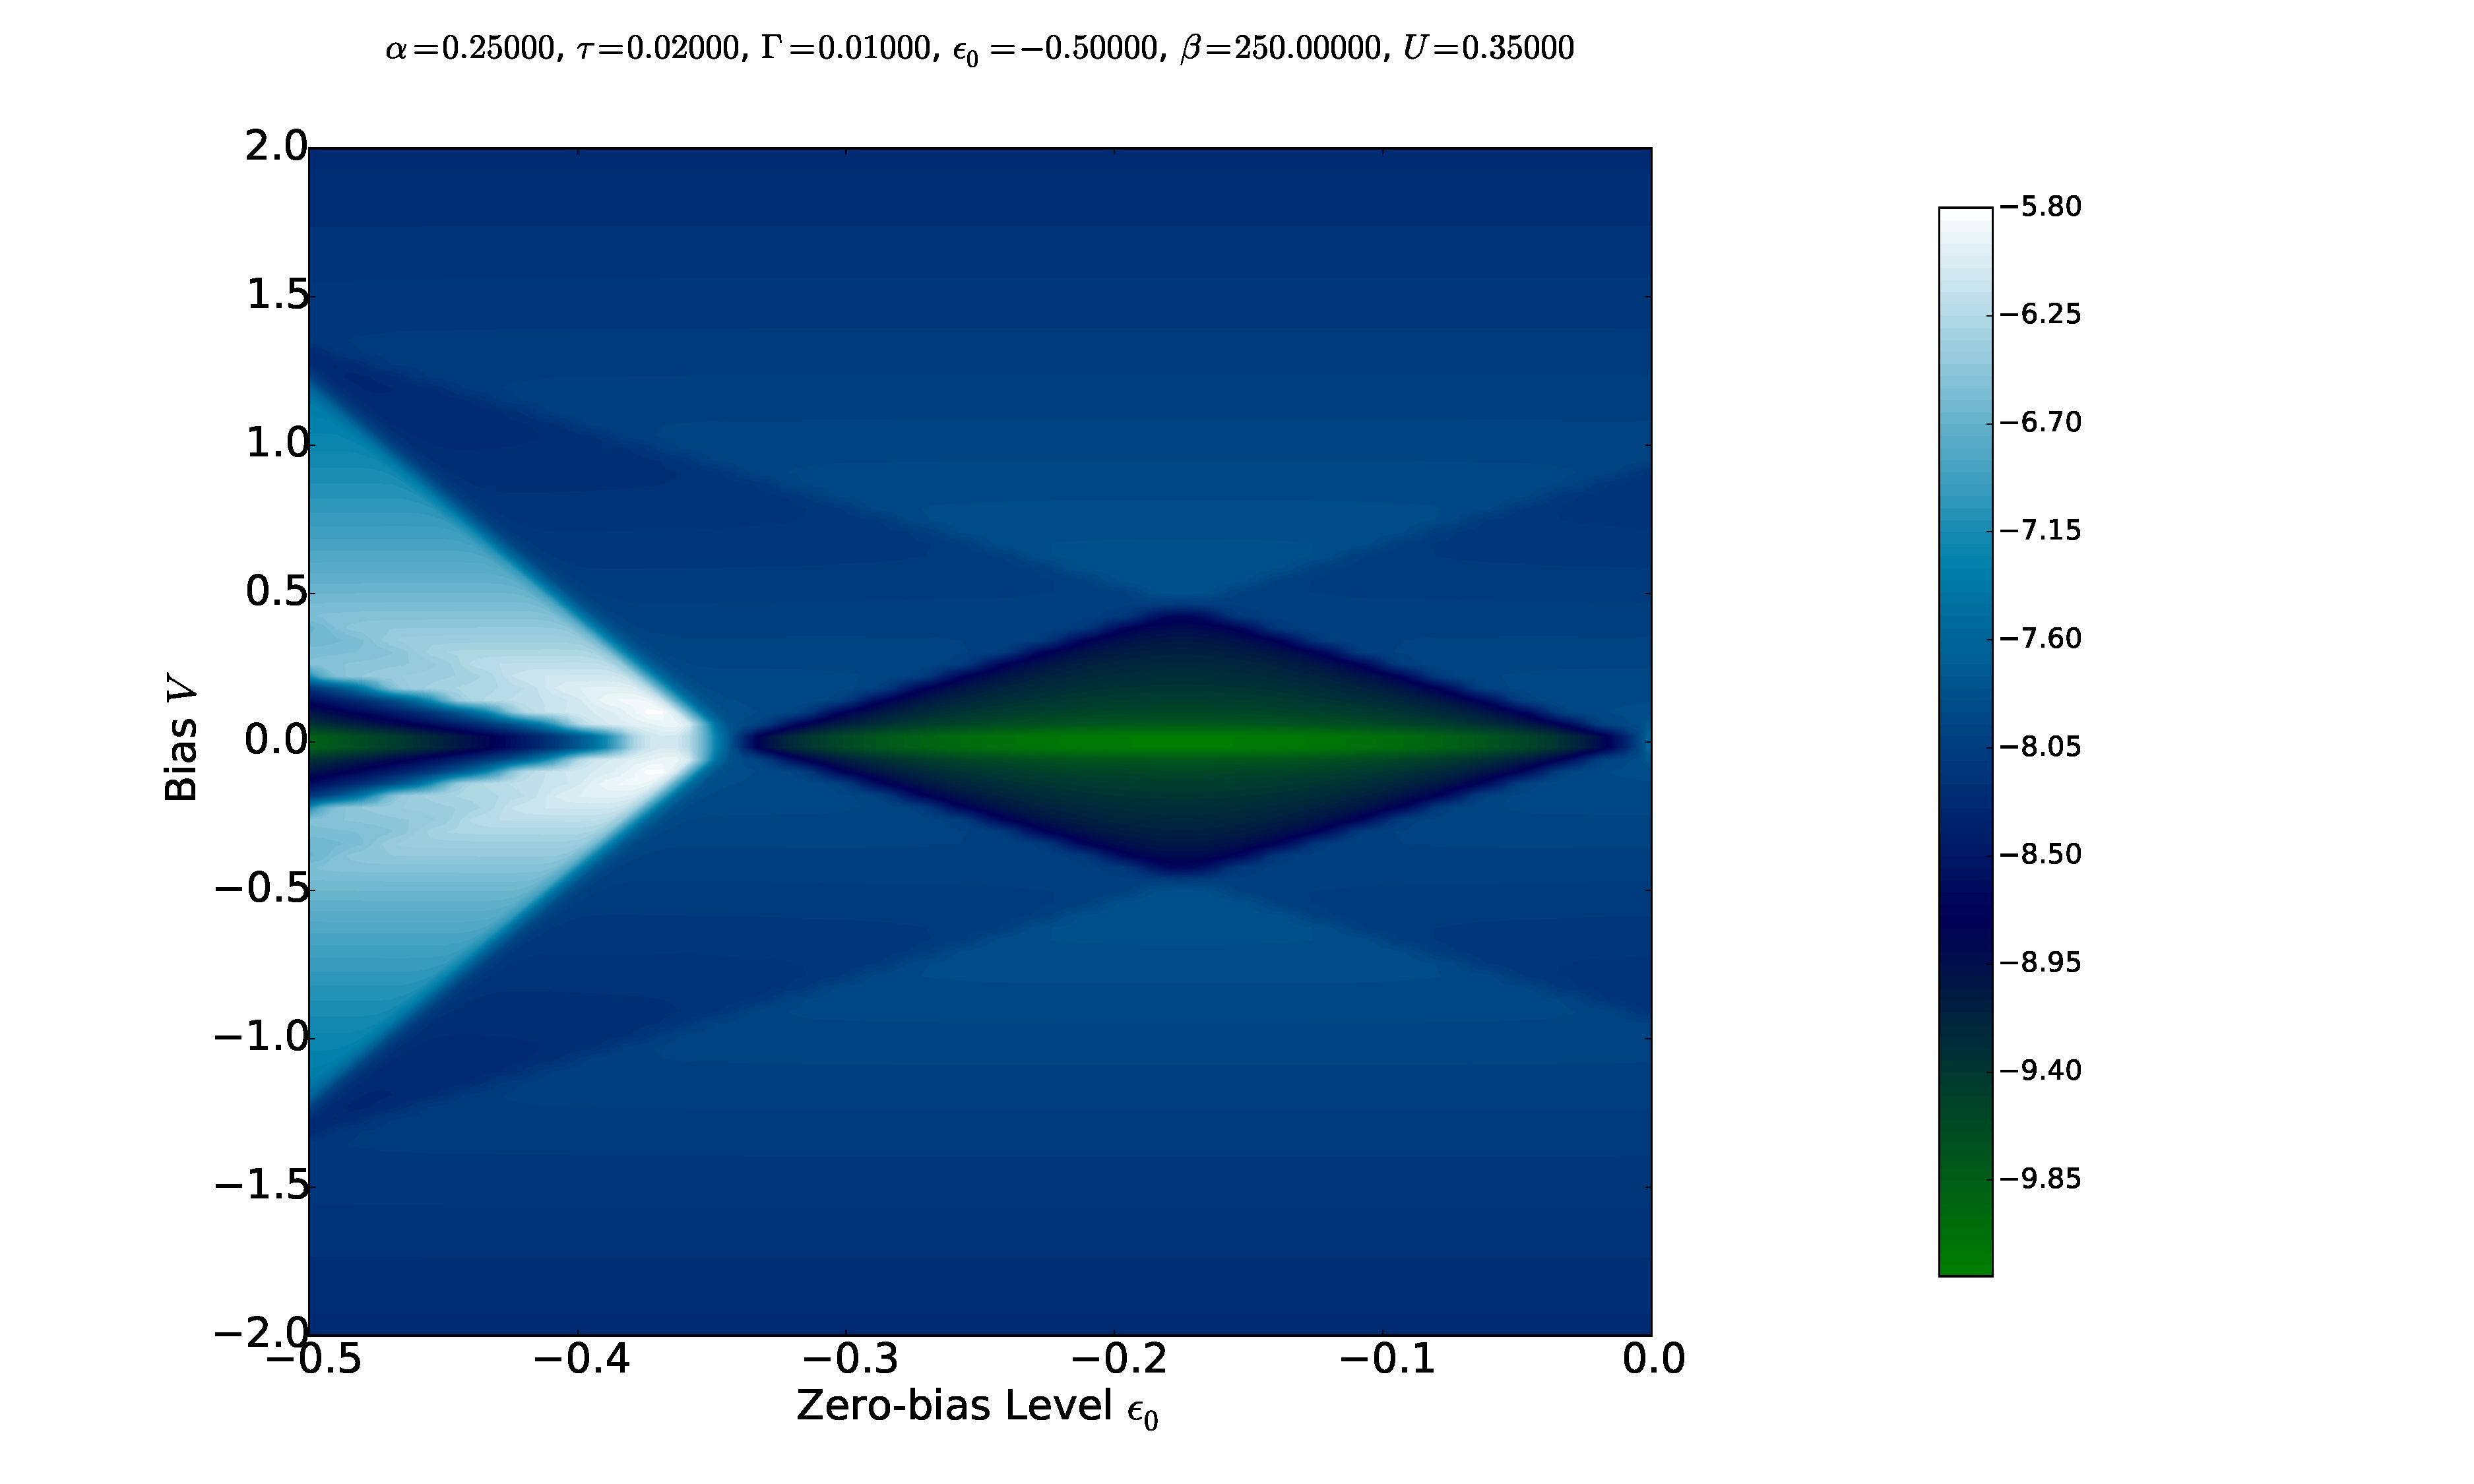
\includegraphics[height=.85\textheight, width=\textwidth]{res/current_map_diamond_alpha_025.pdf}
        \vspace{-6mm}
        \caption{Thin Coulomb Diamond, height depends on $\alpha$.}
    \end{figure} 
\end{frame}
\begin{frame}
    \frametitle{Next}
	\tableofcontents[currentsection,currentsubsection]
\end{frame}
\ssection{Experimental Fit}
\begin{frame}
    \frametitle{Spinless Experimental Fit}
    \vspace{-3mm}
    \begin{figure}[!b] 
        \centering
        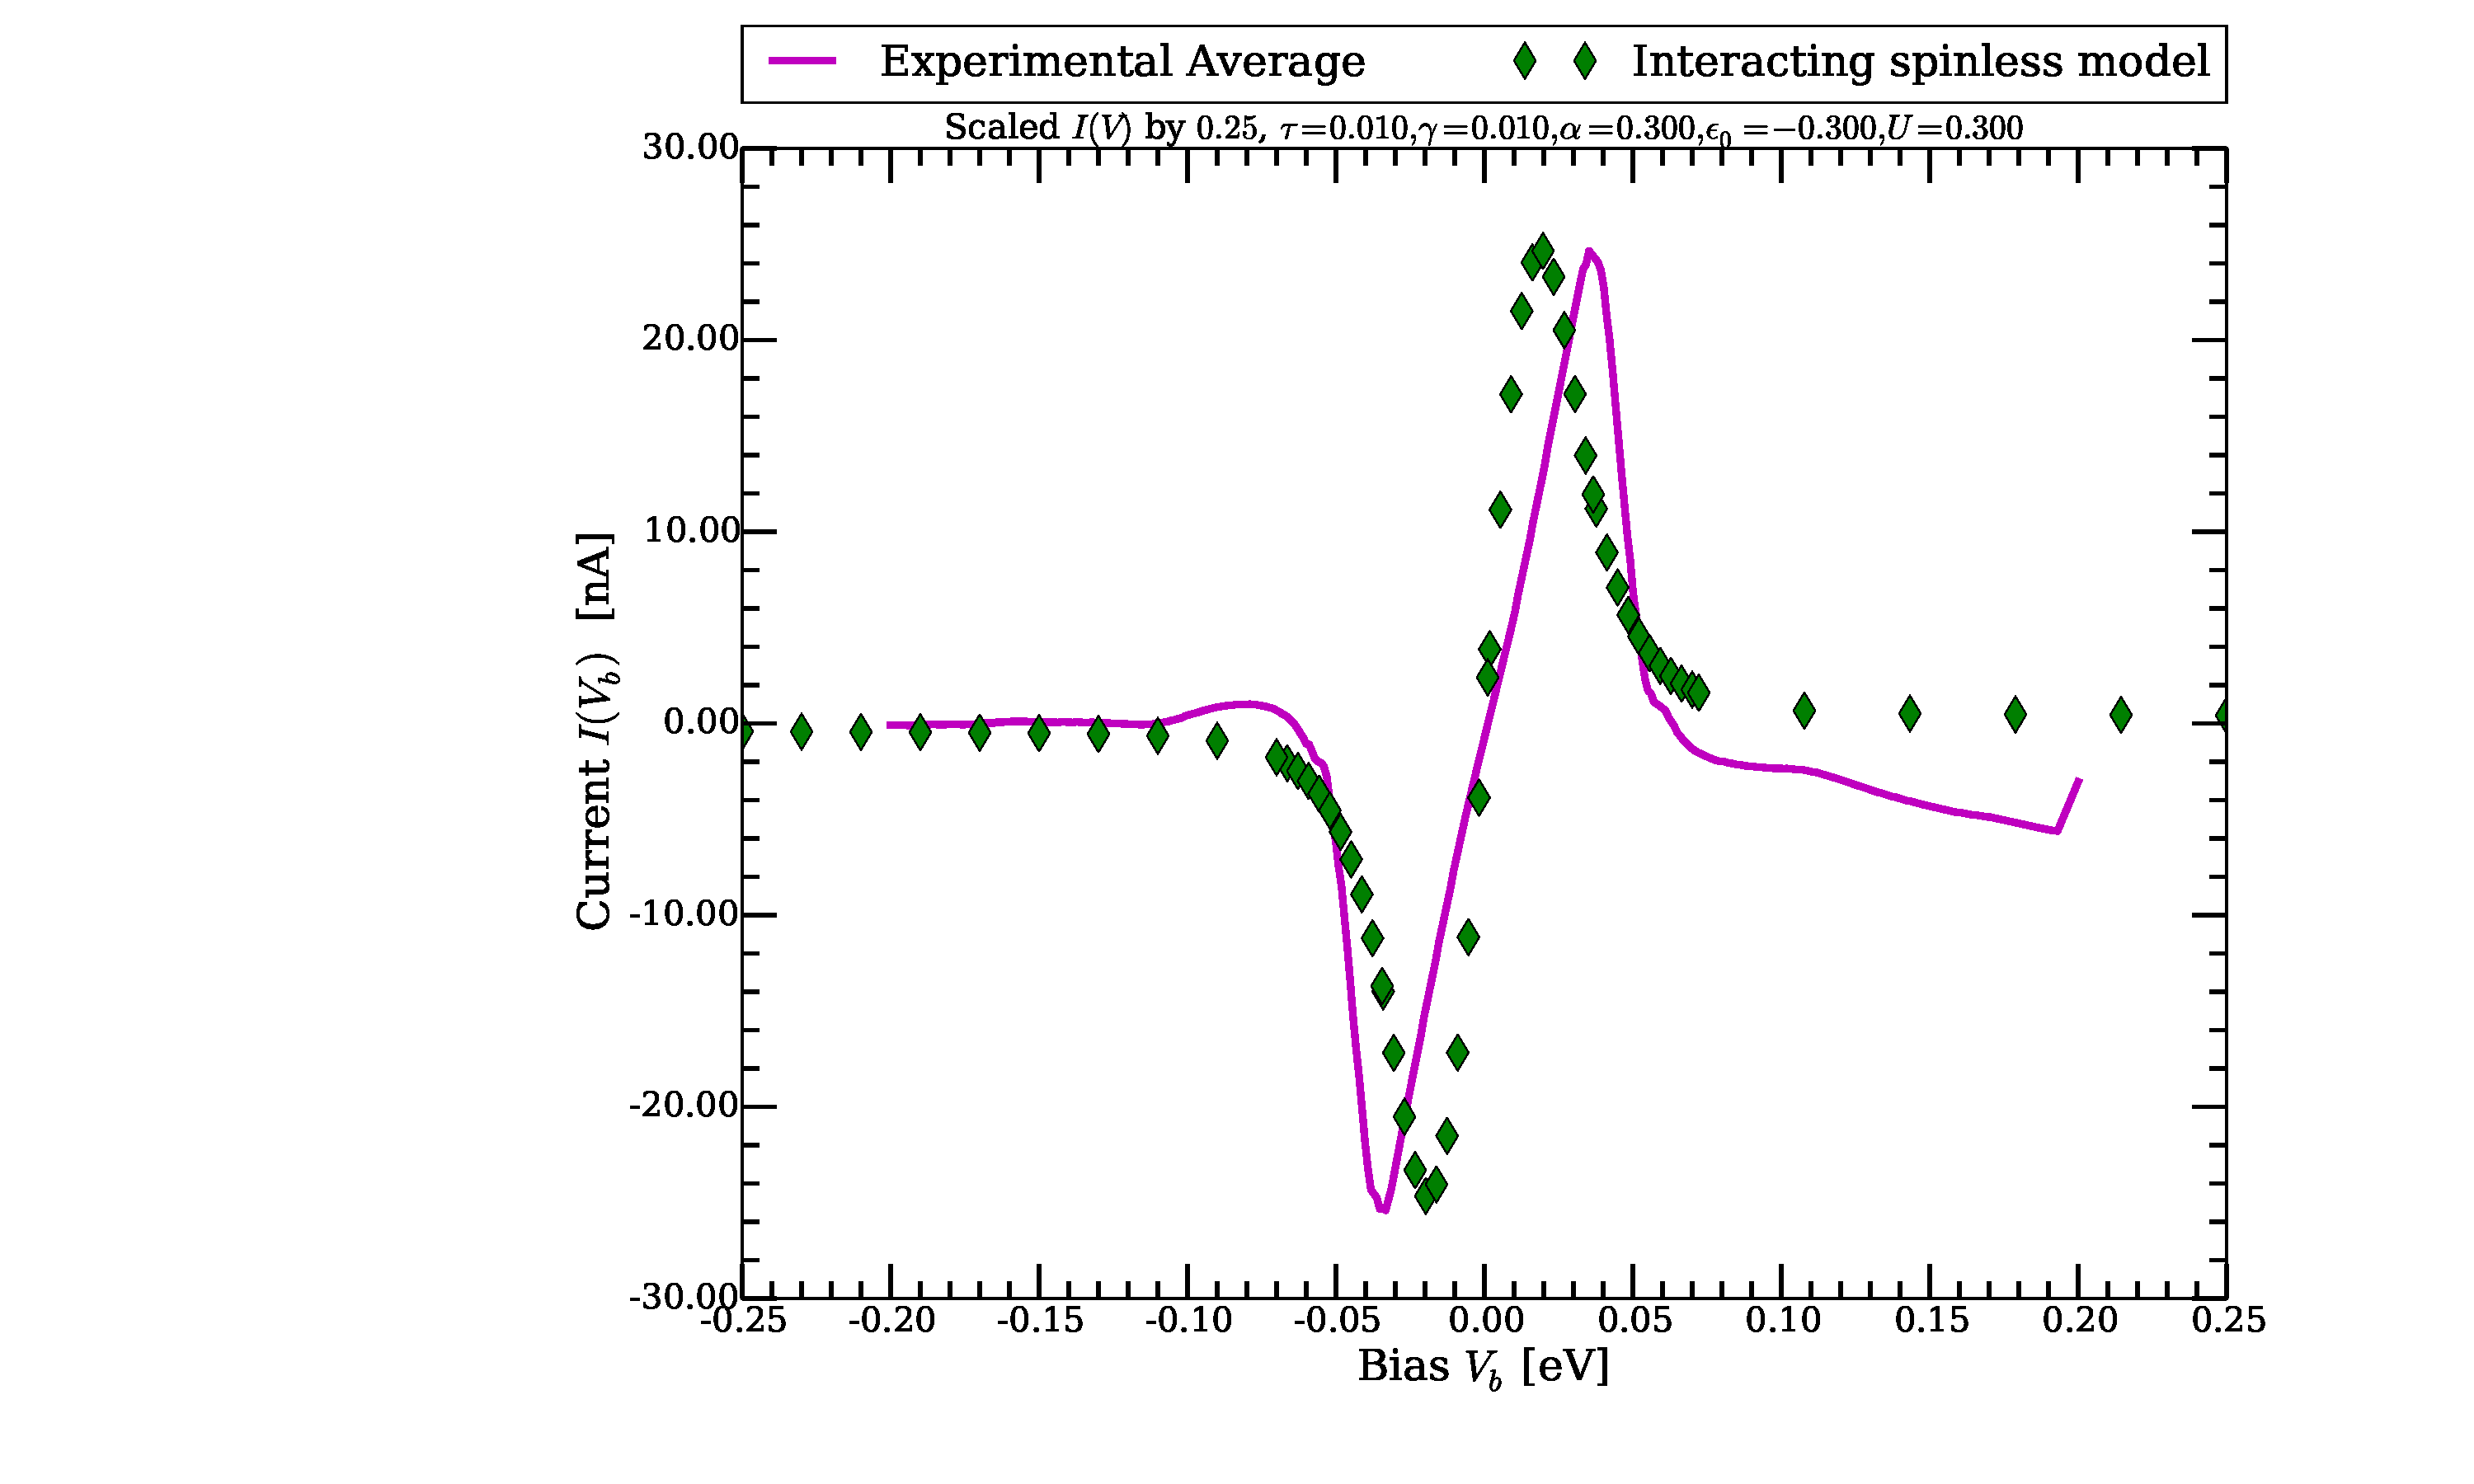
\includegraphics[height=.75\textheight, width=\textwidth, clip=true, trim=6cm 0cm 0cm 0cm]{res/spinless.pdf}
        \vspace{-6mm}
        \caption{Spinless experimental fit.}
    \end{figure} 
\end{frame}
\begin{frame}
    \frametitle{Spinfull Experimental Fit}
    \vspace{-3mm}
    \begin{figure}[!b] 
        \centering
        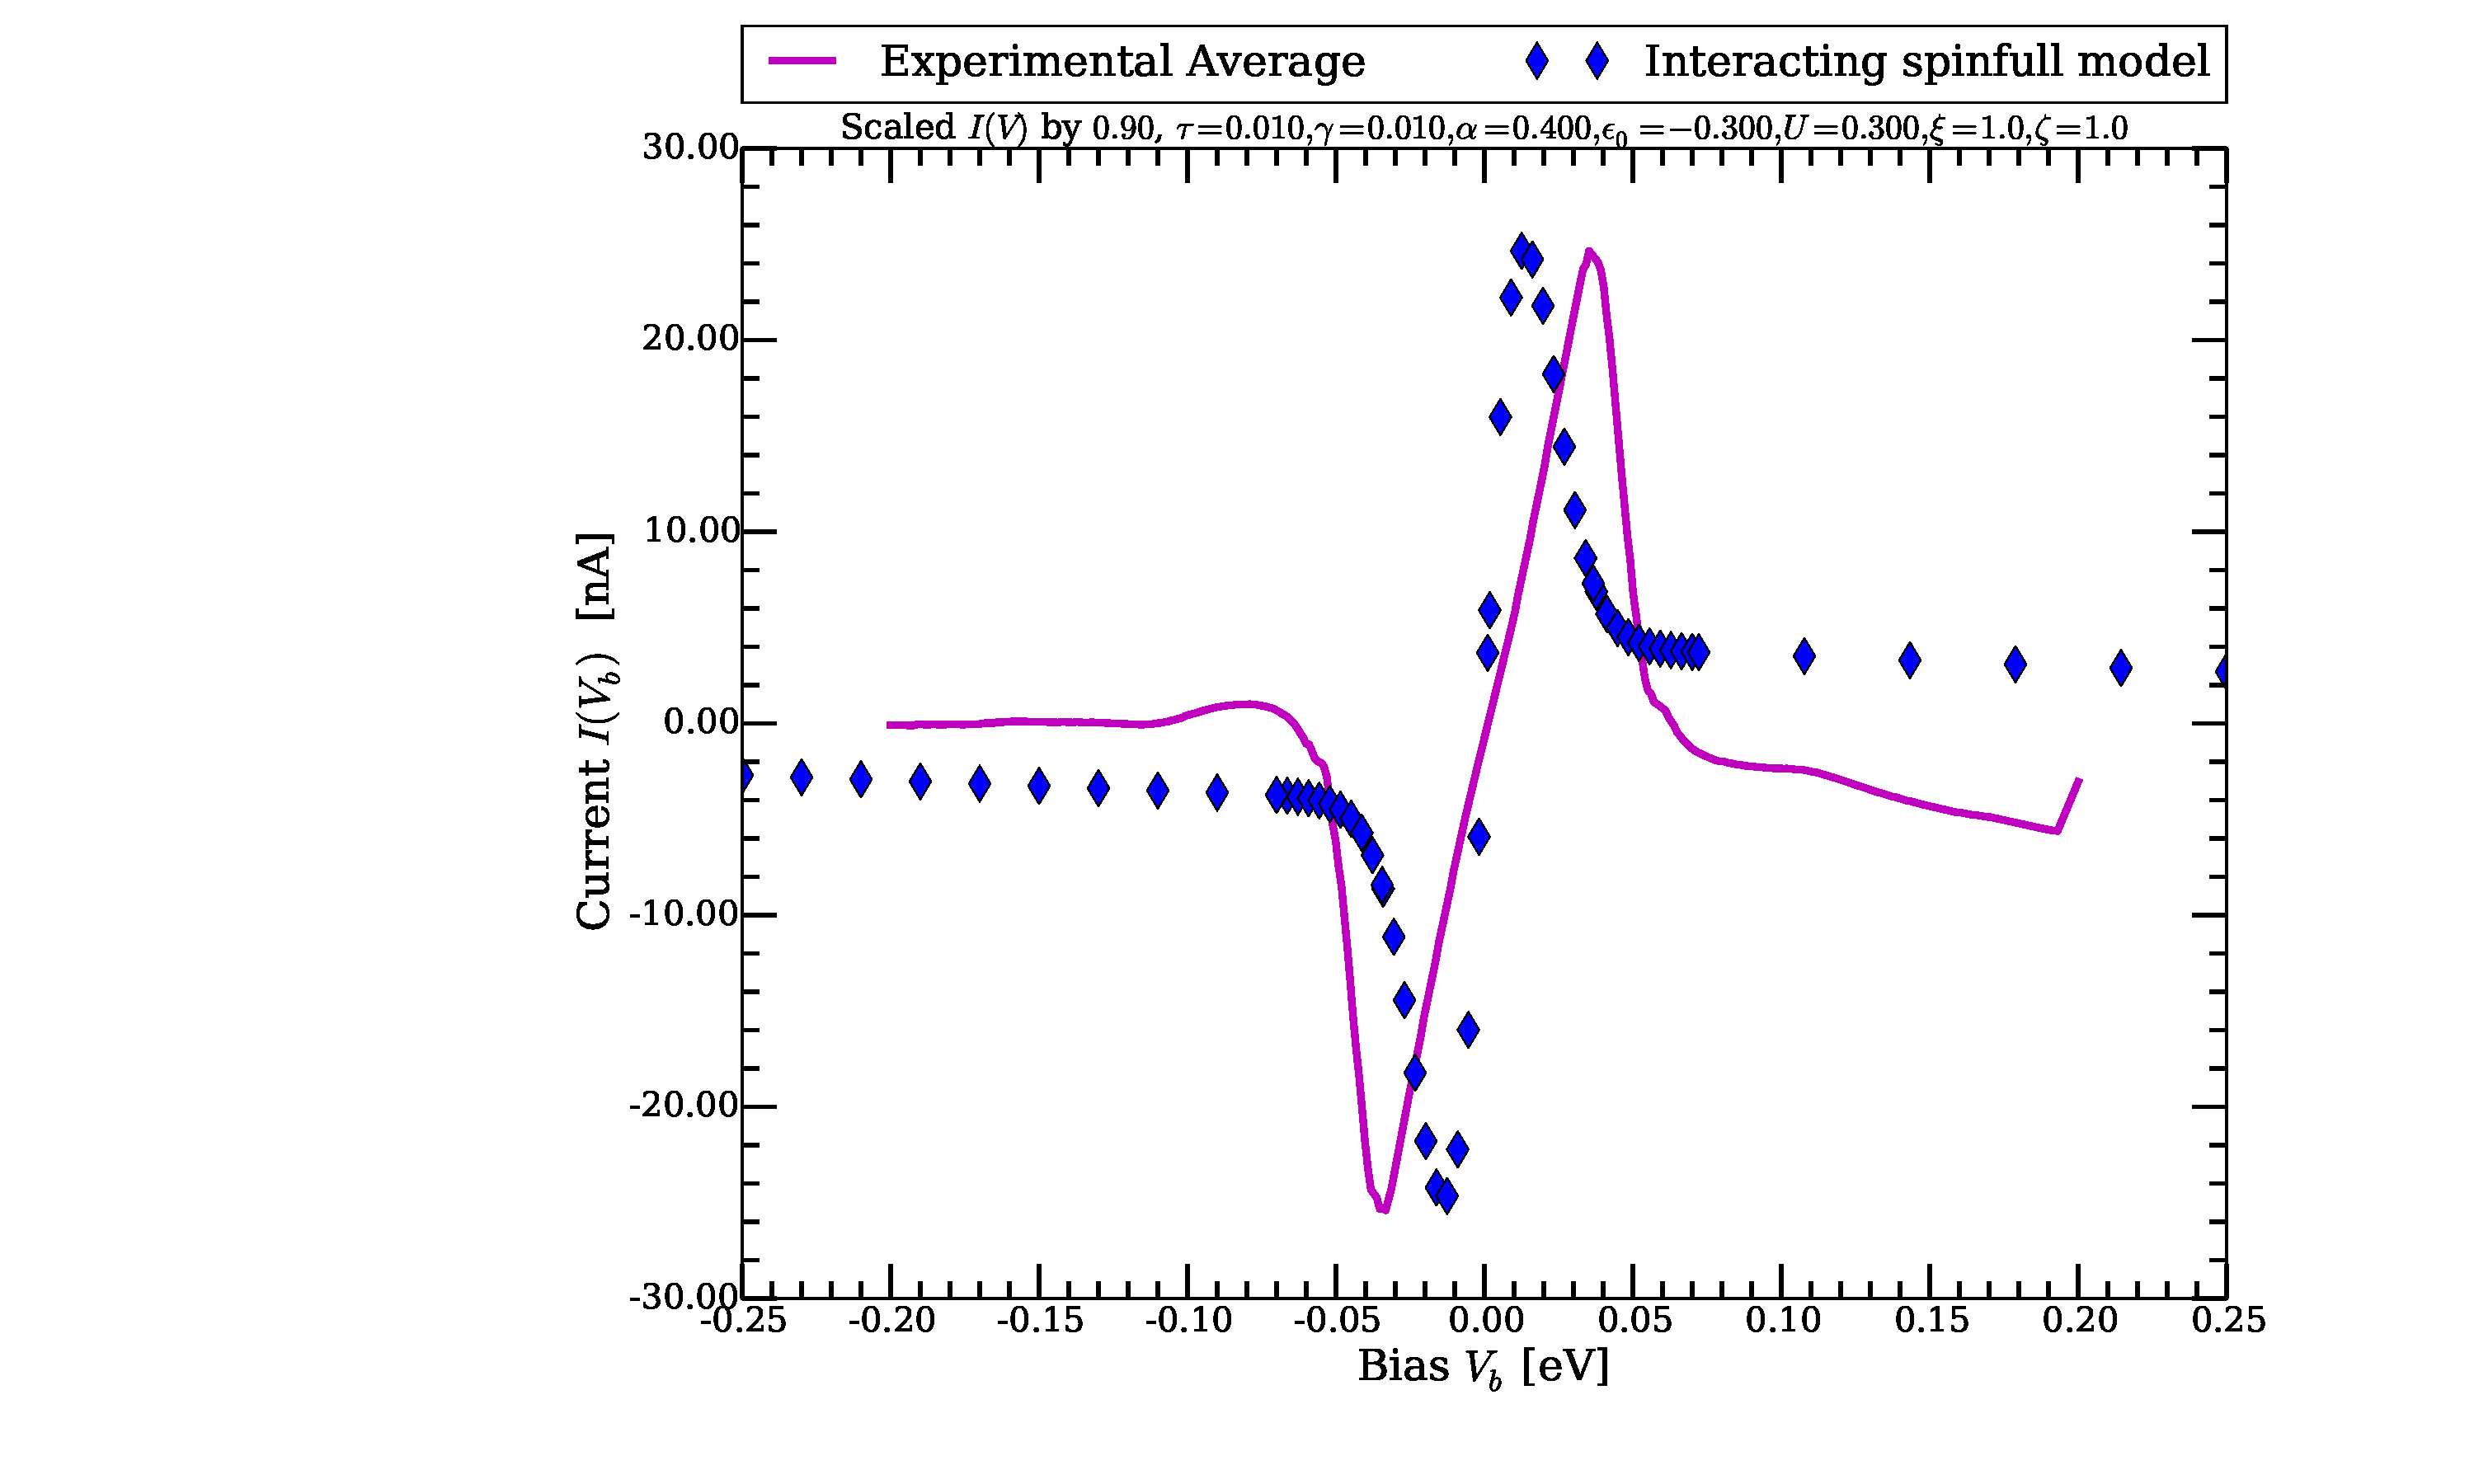
\includegraphics[height=.75\textheight, width=\textwidth]{res/spinfull.pdf}
        \vspace{-6mm}
        \caption{Spinfull experimental fit.}
    \end{figure} 
\end{frame}
\begin{frame}
    \frametitle{Self-Consistent Spinless Experimental Fit}
    \vspace{-3mm}
    \begin{figure}[!b] 
        \centering
        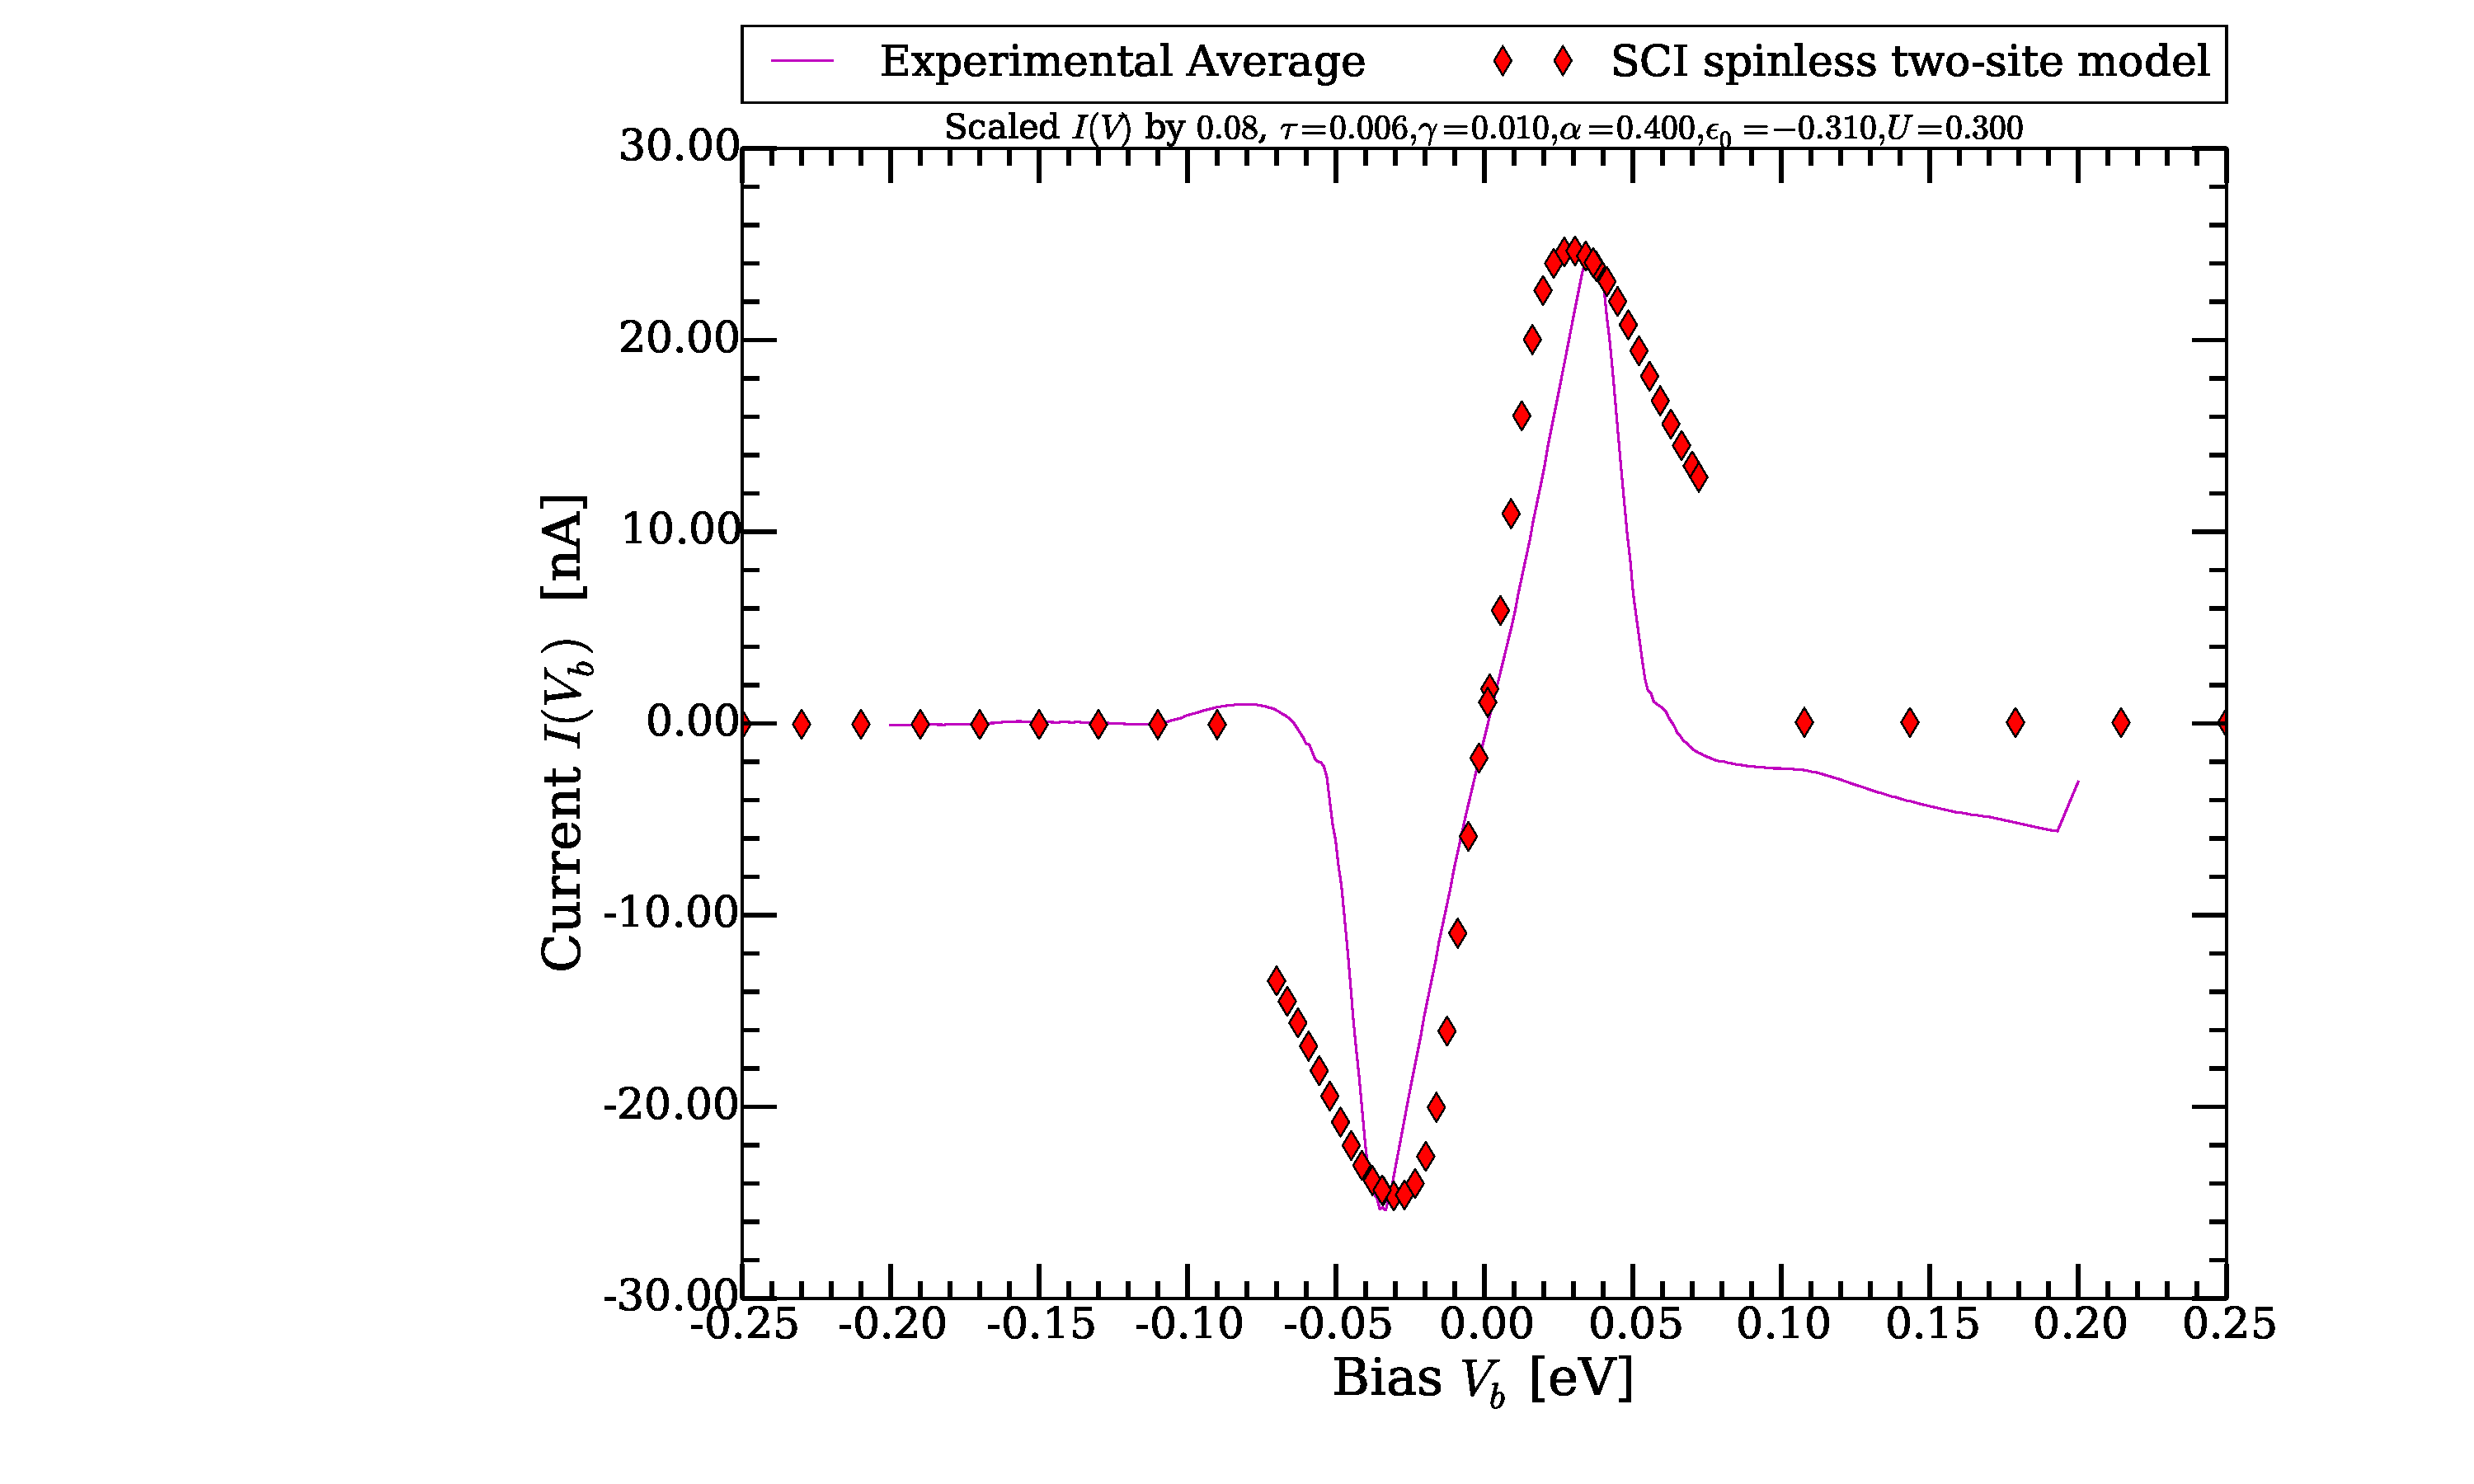
\includegraphics[height=.75\textheight, width=\textwidth]{res/selfconsistent.pdf}
        \vspace{-6mm}
        \caption{Spinfull experimental fit.}
    \end{figure} 
\end{frame}
\section{Conclusions}
\ssection{Summary}
\ssection{Discussion}
\ssection{Future Outlook}